\chapter{Metodología}
\section{Levantamiento de información}
El departamento de ingeniería mecánica en el Campus Casa Central, posee una máquina de fatiga (MF) uniaxial en flexión en el laboratorio de tecnología mecánica que se encuentra en la universidad hace más de 50 años, sin saber su fecha exacta de adquisición. La medición de fatiga es realizada a través del método de \textit{esfuerzo-vida}, utilizando la configuración de \textit{rotating bending}, ambos descritos en el capítulo anterior. La información existente sobre la máquina de ensayos es escasa, principalmente por su antigüedad, la perdida de documentos y obsolescencia de la electrónica. Por lo mismo, parte del trabajo de esta memoria se centra en lograr rescatar información y su posterior comprensión para lograr tener operativa la máquina de fatiga.

\begin{figure}[h]
\centering
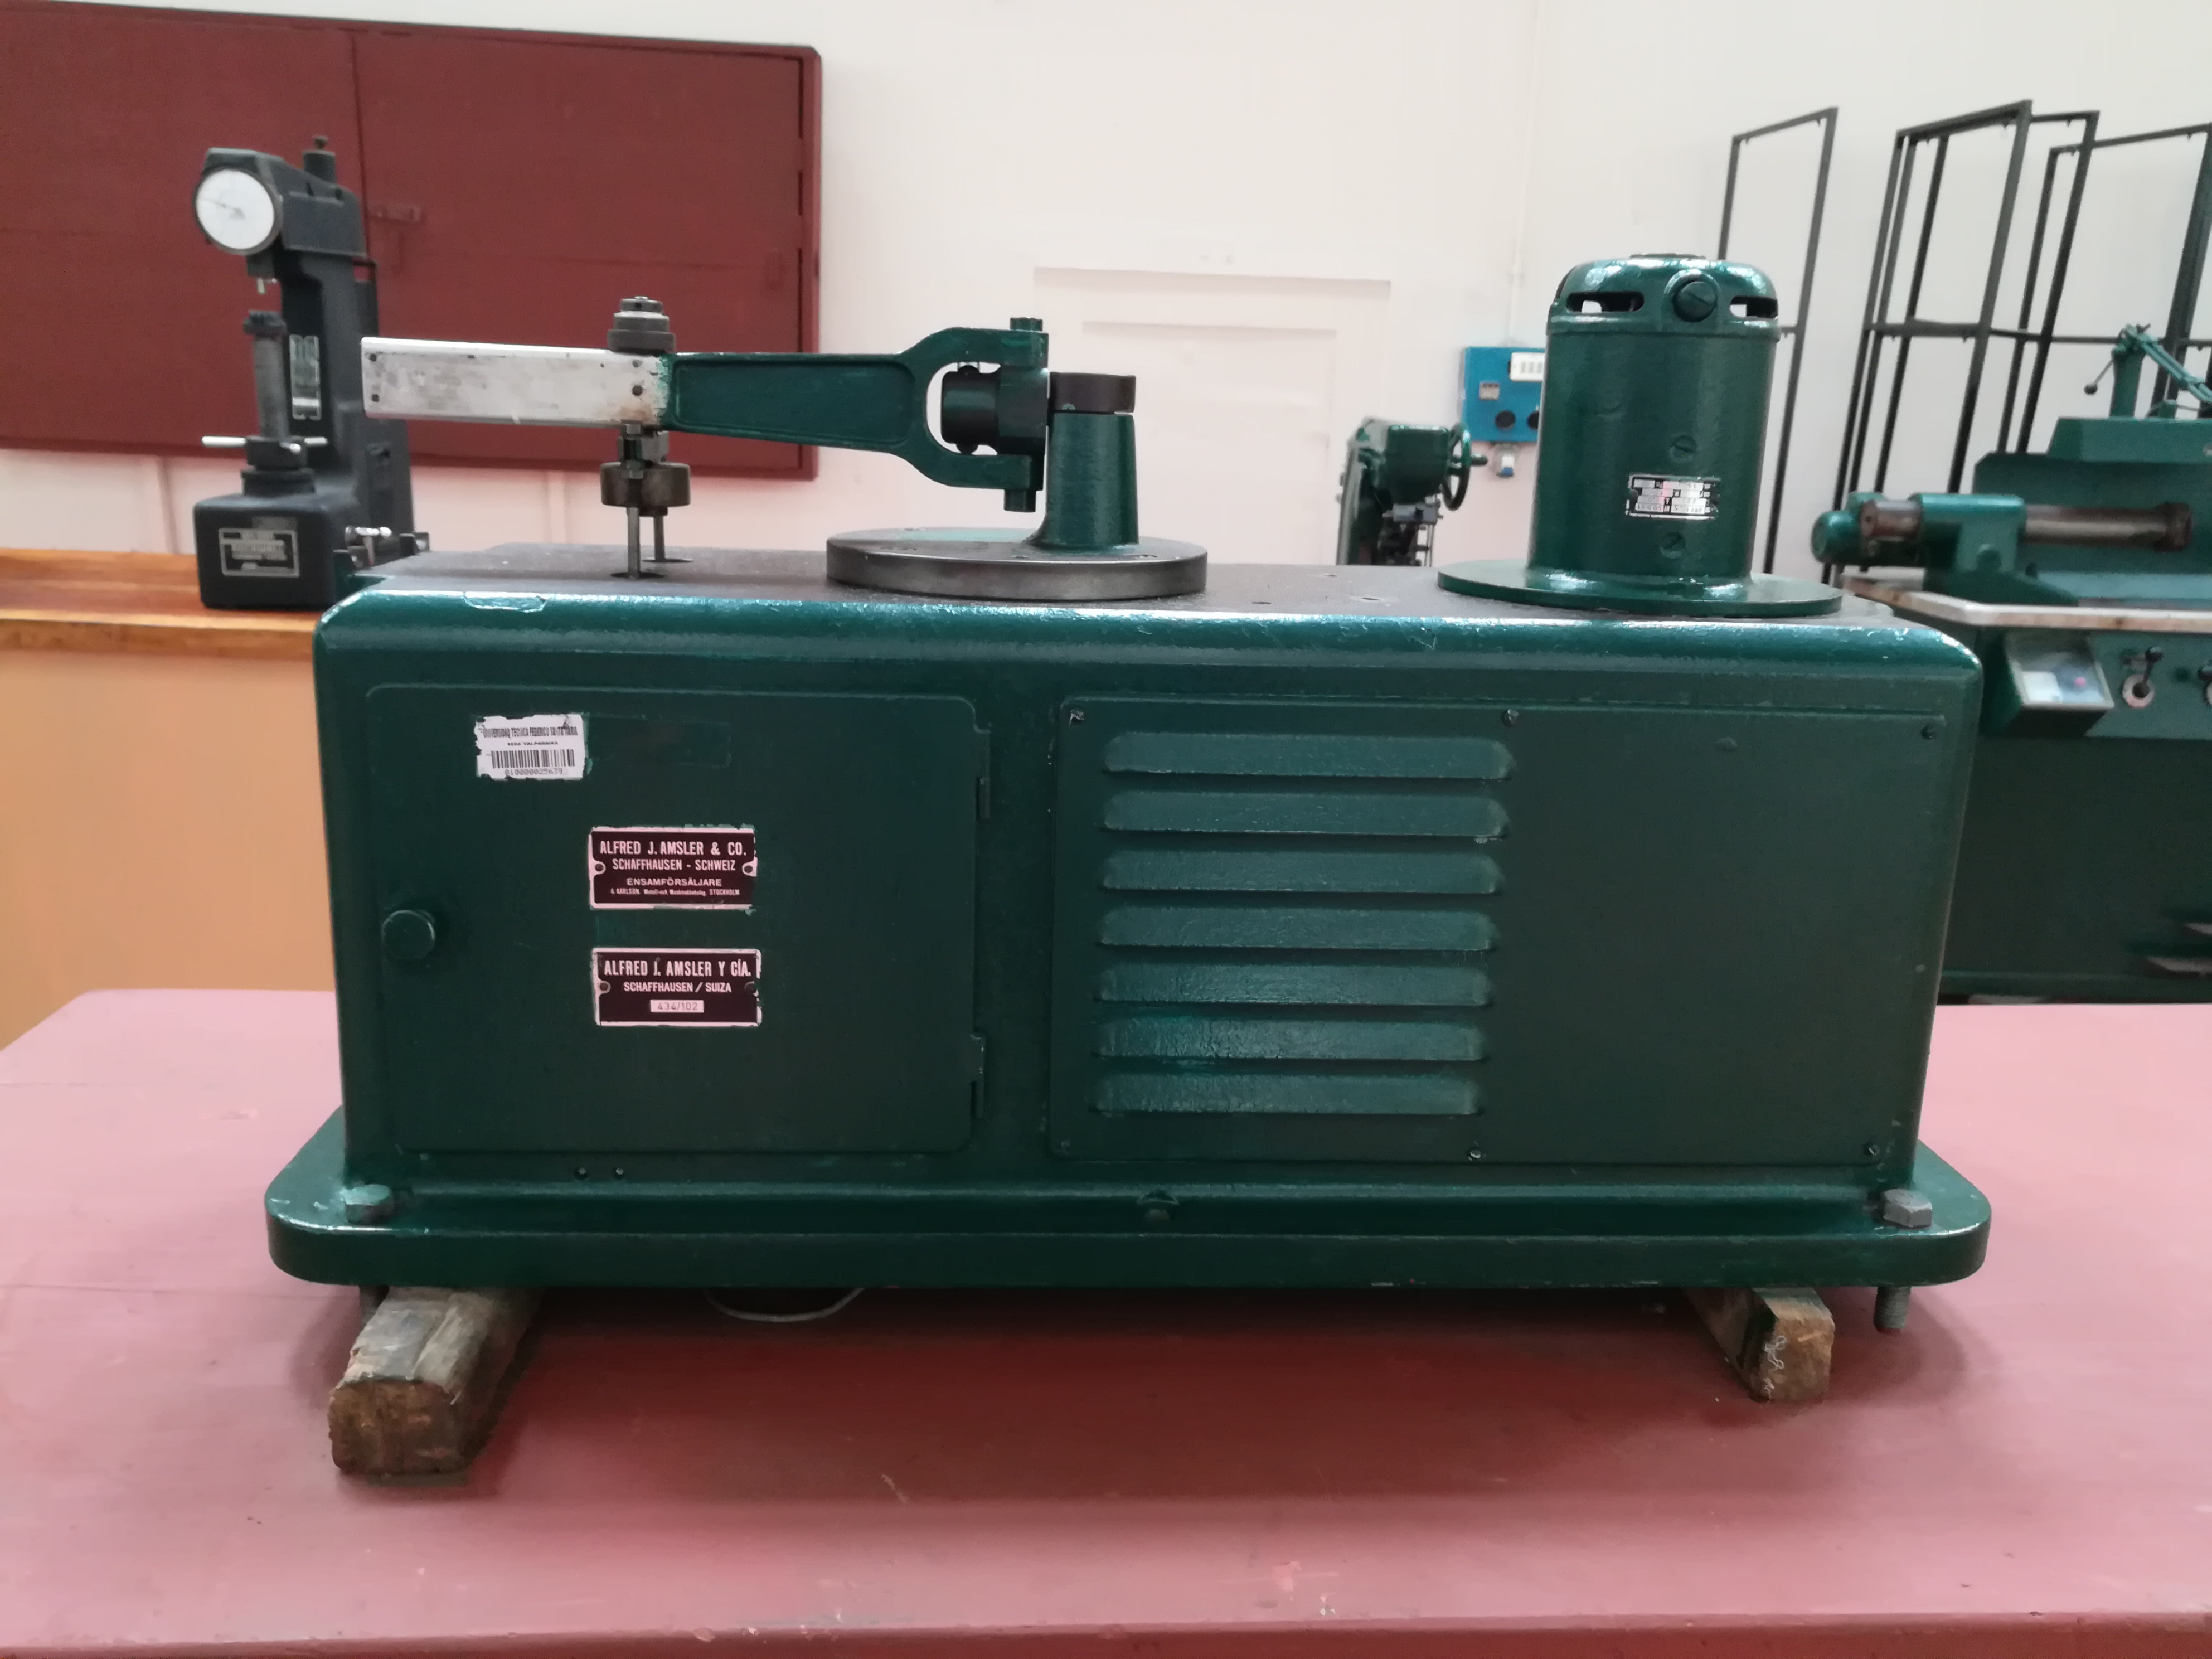
\includegraphics[scale=0.05]{Imagenes/maq_del.jpg}
\label{fig:maq_del}
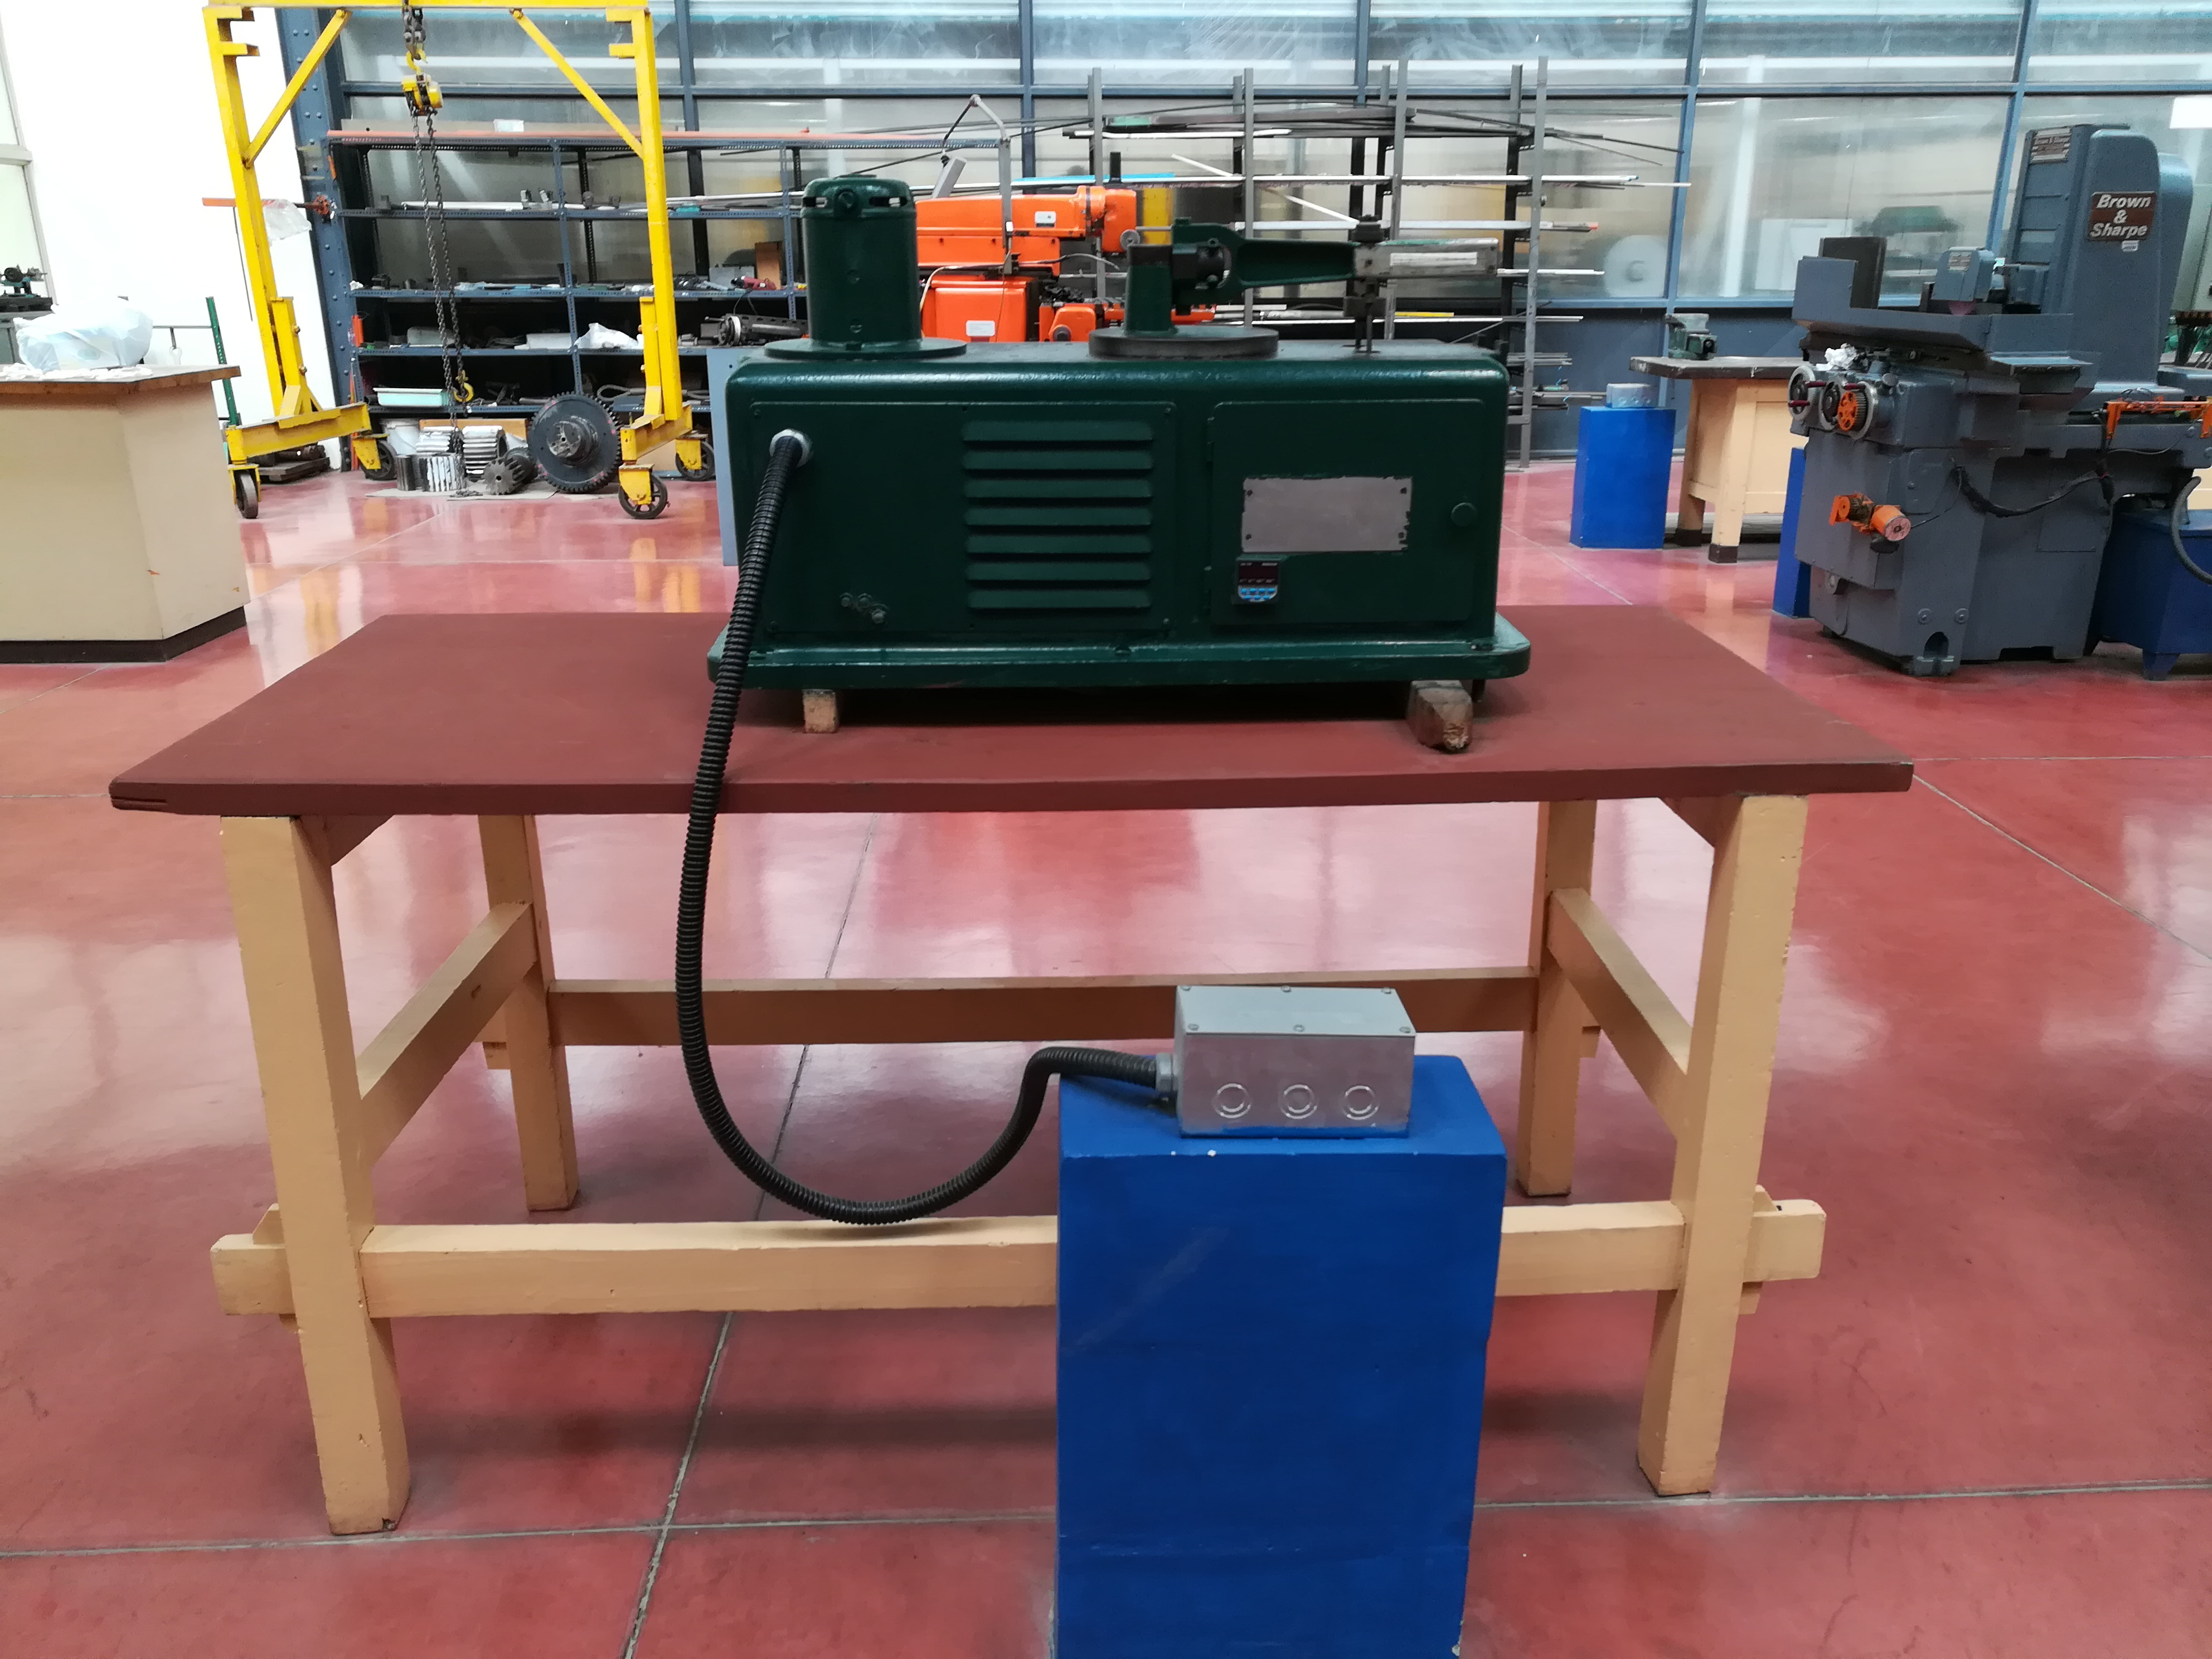
\includegraphics[scale=0.05]{Imagenes/maqfull_post.jpg}
\label{fig:maqfull_post}
\caption{Máquina de fatiga en flexión en el laboratorio de tecnología mecánica}
\label{fig:maq_fat}
\end{figure}

\subsection{Estado actual y antecedentes}
Actualmente la máquina no puede ser utilizada por no estar anclada, estando apoyada sobre dos listones de madera, que a su vez, están sobre una mesa de madera como se aprecia en la figura REF. Por consiguiente, la máquina al ser utilizada comienza a vibrar, saltar y desplazarse lateralmente, lo que impide su uso prolongado por motivos de seguridad. Es decir, no es posible realizar correctamente un ensayo de fatiga de ningún material ni configuración.

A partir de información verbal entregada por el profesor Fernando Rojas, se cree que la máquina fue adquirida por el departamento hace, al menos, 50 años atrás. Fue fabricada en Suiza por \textit{Alfred J. Amsler \& Co.} y su estructura completa es de acero fundido. Previo a la remodelación del piso del laboratorio, la máquina se encontraba anclada al piso con un bloque de concreto que fue demolido durante los trabajos de remodelación, momento desde el cual se encuentra sin una solución definitiva. Más aún, varios equipos y máquinas de ensayo del laboratorio no se encuentran ancladas al piso ni con una instalación definitiva impidiendo su uso.

La única modificación que posee la máquina, según la información recopilada, consiste en el cambio del contador de revoluciones o ciclos realizados en un ensayo de fatiga. Esta actualización consistió en sacar el contador mecánico original y reemplazarlo por un contador electrónico, el cual tiene sus controles y el display adosada a su estructura, como se puede apreciar en la figura \textcolor{red}{agregar imagen del contador}. 

El sistema eléctrico de la máquina permanece intacto, la cual se encuentra conectada a la red de la universidad. Conserva su motor eléctrico original junto a un conjunto eléctrico cuya función es suministrar energía de manera continua y estable al motor, para evitar que el ensayo de fatiga se pueda ver afectado por problemas y las variaciones del suministro eléctrico. El motor es de \textcolor{red}{corriente continua} con velocidad constante y sus especificaciones se pueden ver en la tabla \ref{tab:motor_maq}:

\begin{table}[h]
\centering
\begin{tabular}{ll}
\hline
Especificaciones Motor                            & Valor   				\\ \hline
Tensión                                           & 220 {[}V{]}        		\\
Corriente                                         & 0,8 {[}A{]}        		\\
Factor de potencia ($\cos \varphi$)				  & Sin información    		\\
Potencia                                          & 100 {[}W{]}        		\\
Velocidad                                         & 1500 {[}rev/min{]} 		\\ \hline
\end{tabular}
\caption{Especificaciones del motor de la máquina de fatiga.}
\label{tab:motor_maq}
\end{table}

Otro elemento distinto al original consiste en la correa de transmisión entre el motor eléctrico y el disco desbalanceado. La original consistía en una correa de cuero plana y cruzada, sin información respecto a su empalme. La correa actual consiste también en una correa plana y cruzada, sin embargo, su material es tela y el empalme es realizado a mano con hilo acerado. Cabe destacar que lo poco usual de las dimensiones, características y la necesidad de hacer el empalme en la misma máquina, dificulta la búsqueda de una correa que pueda cumplir de manera óptima la transmisión de potencia. Parte de estas dificultades se deben a que el sistema de transmisión no ha sido modificado donde sus poleas tienen dimensiones, tanto de diámetro como de ancho, que no están normalizadas o se encuentran fuera de catálogo de mucho proveedores. 

Por otro lado, los elementos de agarre de la probeta no tienen modificaciones conocidas, tanto el brazo que recibe el movimiento como el agarre empotrado a la estructura de la máquina. La fabricación de las probetas utilizadas se realiza en el mismo laboratorio a partir de acero AISI 1020 o 1040, el cual para conseguir las dimensiones de la figura REF. se debe cortar y tornear.

Finalmente, para realizar los ensayos en distintas configuraciones existen distintas masas (figura REF) que desequilibran el disco rotativo, como se verá en la sección \ref{sec:funcionamiento}, y estas combinaciones se especifican en una tabla de cargas (Anexo REF). Sin embargo, se desconoce el origen, y en consecuencia, la fiabilidad de la información contenida en esta tabla.

\subsection{Funcionamiento}
\label{sec:funcionamiento}
La máquina de fatiga tiene como objetivo lograr que para cada ciclo se ejerza el mismo esfuerzo determinado sobre la probeta, en forma de flexión. Para lograr esto, el mecanismo utilizado es un disco desequilibrado girando a una velocidad constante $\dot{\theta}$, la fuerza es transmitida hasta un brazo que sostiene a su vez a la probeta, generando flexión en la probeta con un doble empotramiento. La velocidad $\dot{\theta}$ del disco se transmitida desde el motor eléctrico a través de poleas y una correa de transmisión en una relación de 1:1 \textcolor{red}{revisar}, a una velocidad de 1500 revoluciones por minuto. Así, para realizar las mediciones de fatiga a distintas cargas se modifica el desequilibrio del disco a través de un conjunto de masas, mostradas en la figura REF, que permiten generar distintas configuraciones y, por consiguiente, esfuerzos en la probeta.

\textcolor{red}{Agregar imagen de contrapesos}
 c
Los elementos utilizados para desbalancear son 6 discos pequeños de X \textcolor{red}{medir radio masas} a Y de diámetro. Estos son enumerados del 1 al 5, donde el 1 es el más liviano y el 5 el más pesado, todos de distinto peso y el quinto se encuentra repetido. Estas se colocan en los extremos del disco giratorio, como se ve en la figura REFimagendisco, dependiendo de la carga que se desee generar. Para conocer que configuración corresponde a cada esfuerzo aplicado sobre la probeta, se utiliza la tabla de cargas explicada a continuación.


Esta tabla, con 3 columnas de información como se ve en el Anexo REF, nos entrega el esfuerzo normal $\sigma$, cortante $\tau$ y la combinación necesaria para generar esos esfuerzos. Los números entre paréntesis nos indican cuantos contrapesos se deben apilar en cada perno adosado al disco giratorio, los cuales llamaremos soportes de contrapeso (SC). Así, la tabla nos señala que la fuerza es función de la diferencia de masa entre cada soporte, es decir, la suma de las masas de cada paréntesis. A modo de ejemplo, en la tabla \ref{tab:ejemplo_config} se han colocado las 4 primeras filas de la tabla de cargas, añadiendo 4 columnas con información sobre el peso de cada combinación. En las columnas $m_1$ y $m_2$ se aprecia la suma de cada masa colocada en sus soportes de contrapeso señalado por la columna de ``Combinación''. Las columnas siguientes representan $\Delta m = m_1-m_2$ y $m_{total}=m_1+_2$. Como se puede apreciar, los esfuerzos normales y cortantes aumentan en la medida que $\Delta m$ de cada combinación aumenta, independiente de $m_{total}$.

\begin{table}[h]
\centering
\label{tab:ejemplo_config}
\begin{tabular}{@{}cclllll@{}}
\toprule
$\sigma \left[\frac{\text{kg}_f}{\text{cm}^2}\right]$ & {$\tau \left[\frac{\text{kg}_f}{\text{cm}^2}\right]$} & Combinación     & $m_1$ {[}g{]} & $m_2$ {[}g{]} & $\Delta m$ {[}g{]} & $m_{total}$ {[}g{]} \\ \midrule
40                                                   & 20                                                                    & (5) - (1+2+3+4) & 30,9199       & 30,5071       & 0,4128             & 61,427              \\
80                                                   & 40                                                                    & (1) - (0)       & 0,7582        & 0             & 0,7582             & 0,7582              \\
120                                                  & 60                                                                    & (5) - (4+2+3)   & 30,9199       & 29,7489       & 1,171              & 60,6688             \\
160                                                  & 80                                                                    & (2) - (1)       & 2,2969        & 0,7582        & 1,5387             & 3,0551              \\ \bottomrule
\end{tabular}
\caption{Tabla de configuración de las masas modificada, mostrando el peso, su diferencia y el total para cada combinación}
\end{table}

Con esto, la probeta a ensayar estará sometida a un esfuerzo en flexión, empotrada en ambos lados por la mordaza del brazo y la mordaza empotrada a la estructura de la máquina, ambas mostradas en la figura REF. Una vez que se haya escogido la configuración de masas y la probeta se encuentre en su posición, una pequeña barra con una manilla ubicada entre las barras de acero, como se aprecia en la figura REF, eleva ambas barras con el objetivo de evitar que oscile durante el encendido y aceleración del motor hasta su velocidad final, dejando a la barra en una configuración de empotrado y apoyo simple. Una vez que el motor alcanza una velocidad estable, el sostén es girado nuevamente para dejar al disco giratorio en posición de empotrado-libre. Este sostén, permite que el ensayo de fatigue se realice siempre a una frecuencia constante y evitar la transición inicial del motor. Una vez que la probeta se fracture, provocarán un aumento en la amplitud de las oscilaciones del disco las cuales activarán el freno automático (figura REF) para detener el motor y, por lo tanto, el ensayo. Gracias a este sistema, es posible conocer la cantidad de ciclos que realizados hasta el momento de fractura sin la necesidad de supervisar de manera continua el ensayo.

\textcolor{red}{Mordazas}
\subsection{Mediciones}
Para realizar un correcto diseño de la estructura soportante y la comprensión de su funcionamiento, se hace vital poder contar con información confiable para obtener resultados correctos. Para esto, las mediciones se dividirán según su objetivo en el desarrollo de este trabajo.
\subsubsection{Diseño de estructura}
Las medidas de la mesa actual son: 
\begin{itemize}
	\item Ancho = 74,5 cm
	\item Largo = 177 cm
	\item Altura = 91 cm
\end{itemize}
Por otro lado, para diseñar correctamente la estructura se deben conocer las dimensiones de la máquina, su peso y la ubicación de los pernos de anclaje, así como también el tipo de perno utilizado. La figura REF\textcolor{red}{realizar diagrama con vistas frontal y lateral de la maquina con sus dimensiones} es un esquema representativo de la máquina, mostrando sus dimensiones de ancho, alto y largo, las dimensiones de su base y la ubicación de sus pernos. La masa de toda la máquina se aproximó a partir de las dimensiones externas, estimando el grosor de sus paredes y considerando el peso específico del acero fundido, sobrestimando el valor del espesor de sus paredes como factor de seguridad. Considerando el peso específico del acero $\rho_{acfund} = 7850 \, [Kg/m^3]$, entonces la masa total calculada es:

\[ \left. 
\begin{array}{ll}
V_{base} &= (3,3\cdot 91\cdot 39 - 3\cdot 88\cdot 37)\; \text{cm}^3	\\
V_{superior} &=(30,2\cdot 84\cdot 32 - 26\cdot 78\cdot 28,5) \; \text{cm}^3	\\
\end{array}
\right\} \\
\quad V_{b+s} = 25323,3 \; \text{cm}^3 \]
\begin{equation}
	m_{maq} = \rho_{ac. fundido} \cdot V_{b+s} = 198,8 \: kg \approx 200 \: kg
\end{equation}

\subsubsection{Componentes de la máquina de fatiga}
\subparagraph{Sistema de transmisión.}
El sistema de transmisión está compuesto por el motor eléctrico, cuyas características se detallaron anteriormente, la correa de transmisión y ambas poleas. Las dimensiones y características de las poleas conductora y conducida, como también de la correa se encuentran en la tabla \ref{tab:sist_transmision}. 

\begin{table}[h]
\centering
\begin{tabular}{@{}ll@{}}
\toprule
Características          & Valor   			\\ \midrule
Diámetro polea motriz    & 48 mm   			\\
Diámetro polea conducida & 47,5 mm 			\\
Relación de poleas		 & $\approx$ 1 (-) 	\\
Ancho correa             & 10 mm   			\\
Longitud correa          & 1235 mm 			\\
Configuración            & Cruzada 			\\ \bottomrule
\end{tabular}
\caption{Datos del sistema de transmisión}
\label{tab:sist_transmision}
\end{table}

\subparagraph{Barras de acero.}
El conjunto de barras de acero que sostienen el disco en empotrado-libre, tienen medidas levemente distintas para las superiores respecto a las inferiores, separadas por una distancia de 32 mm. La tabla \ref{tab:medidas_barrasacero} muestra las medidas de cada una.
\begin{table}[h]
\centering
\begin{tabular}{@{}lll@{}}
\toprule
Medida  & Barras superiores {[}mm{]} & Barras inferiores {[}mm{]} \\ \midrule
Espesor      & 5,7                        & 5,8                        \\
Ancho        & 25,1                       & 25,2                       \\
Largo        & 333                        & 333                        \\ \bottomrule
\end{tabular}
\caption{Medidas de las barras de acero según su posición}
\label{tab:medidas_barrasacero}
\end{table}

Con estos datos, es posible calcular el segundo momento de área respecto a un eje central horizontal equidistante entre las barras superiores e inferiores, según el cual es obtiene $I=asfaf$. 

\subparagraph{Sistema de transmisión de fuerzas.}
El brazo principal (figura \ref{fig:brazo_carga}) que ejerce la fuerza sobre la probeta proveniente del disco desbalanceado, está constituido por tres partes principales. La primera de ellas es la parte trasera, con forma regular rectangular, está hecho de una aleación de aluminio y dos tercios de su longitud es ahuecada. La segunda y principal, está hecha de acero fundido y añade el mayor porcentaje de masa al total del brazo. Finalmente, la última parte consiste en la mordaza, unida a la sección principal con dos pernos que permiten ajustar su posición. La longitud total del brazo es de 359 mm y su masa total 2,305 kg.

\begin{figure}[h]
\centering
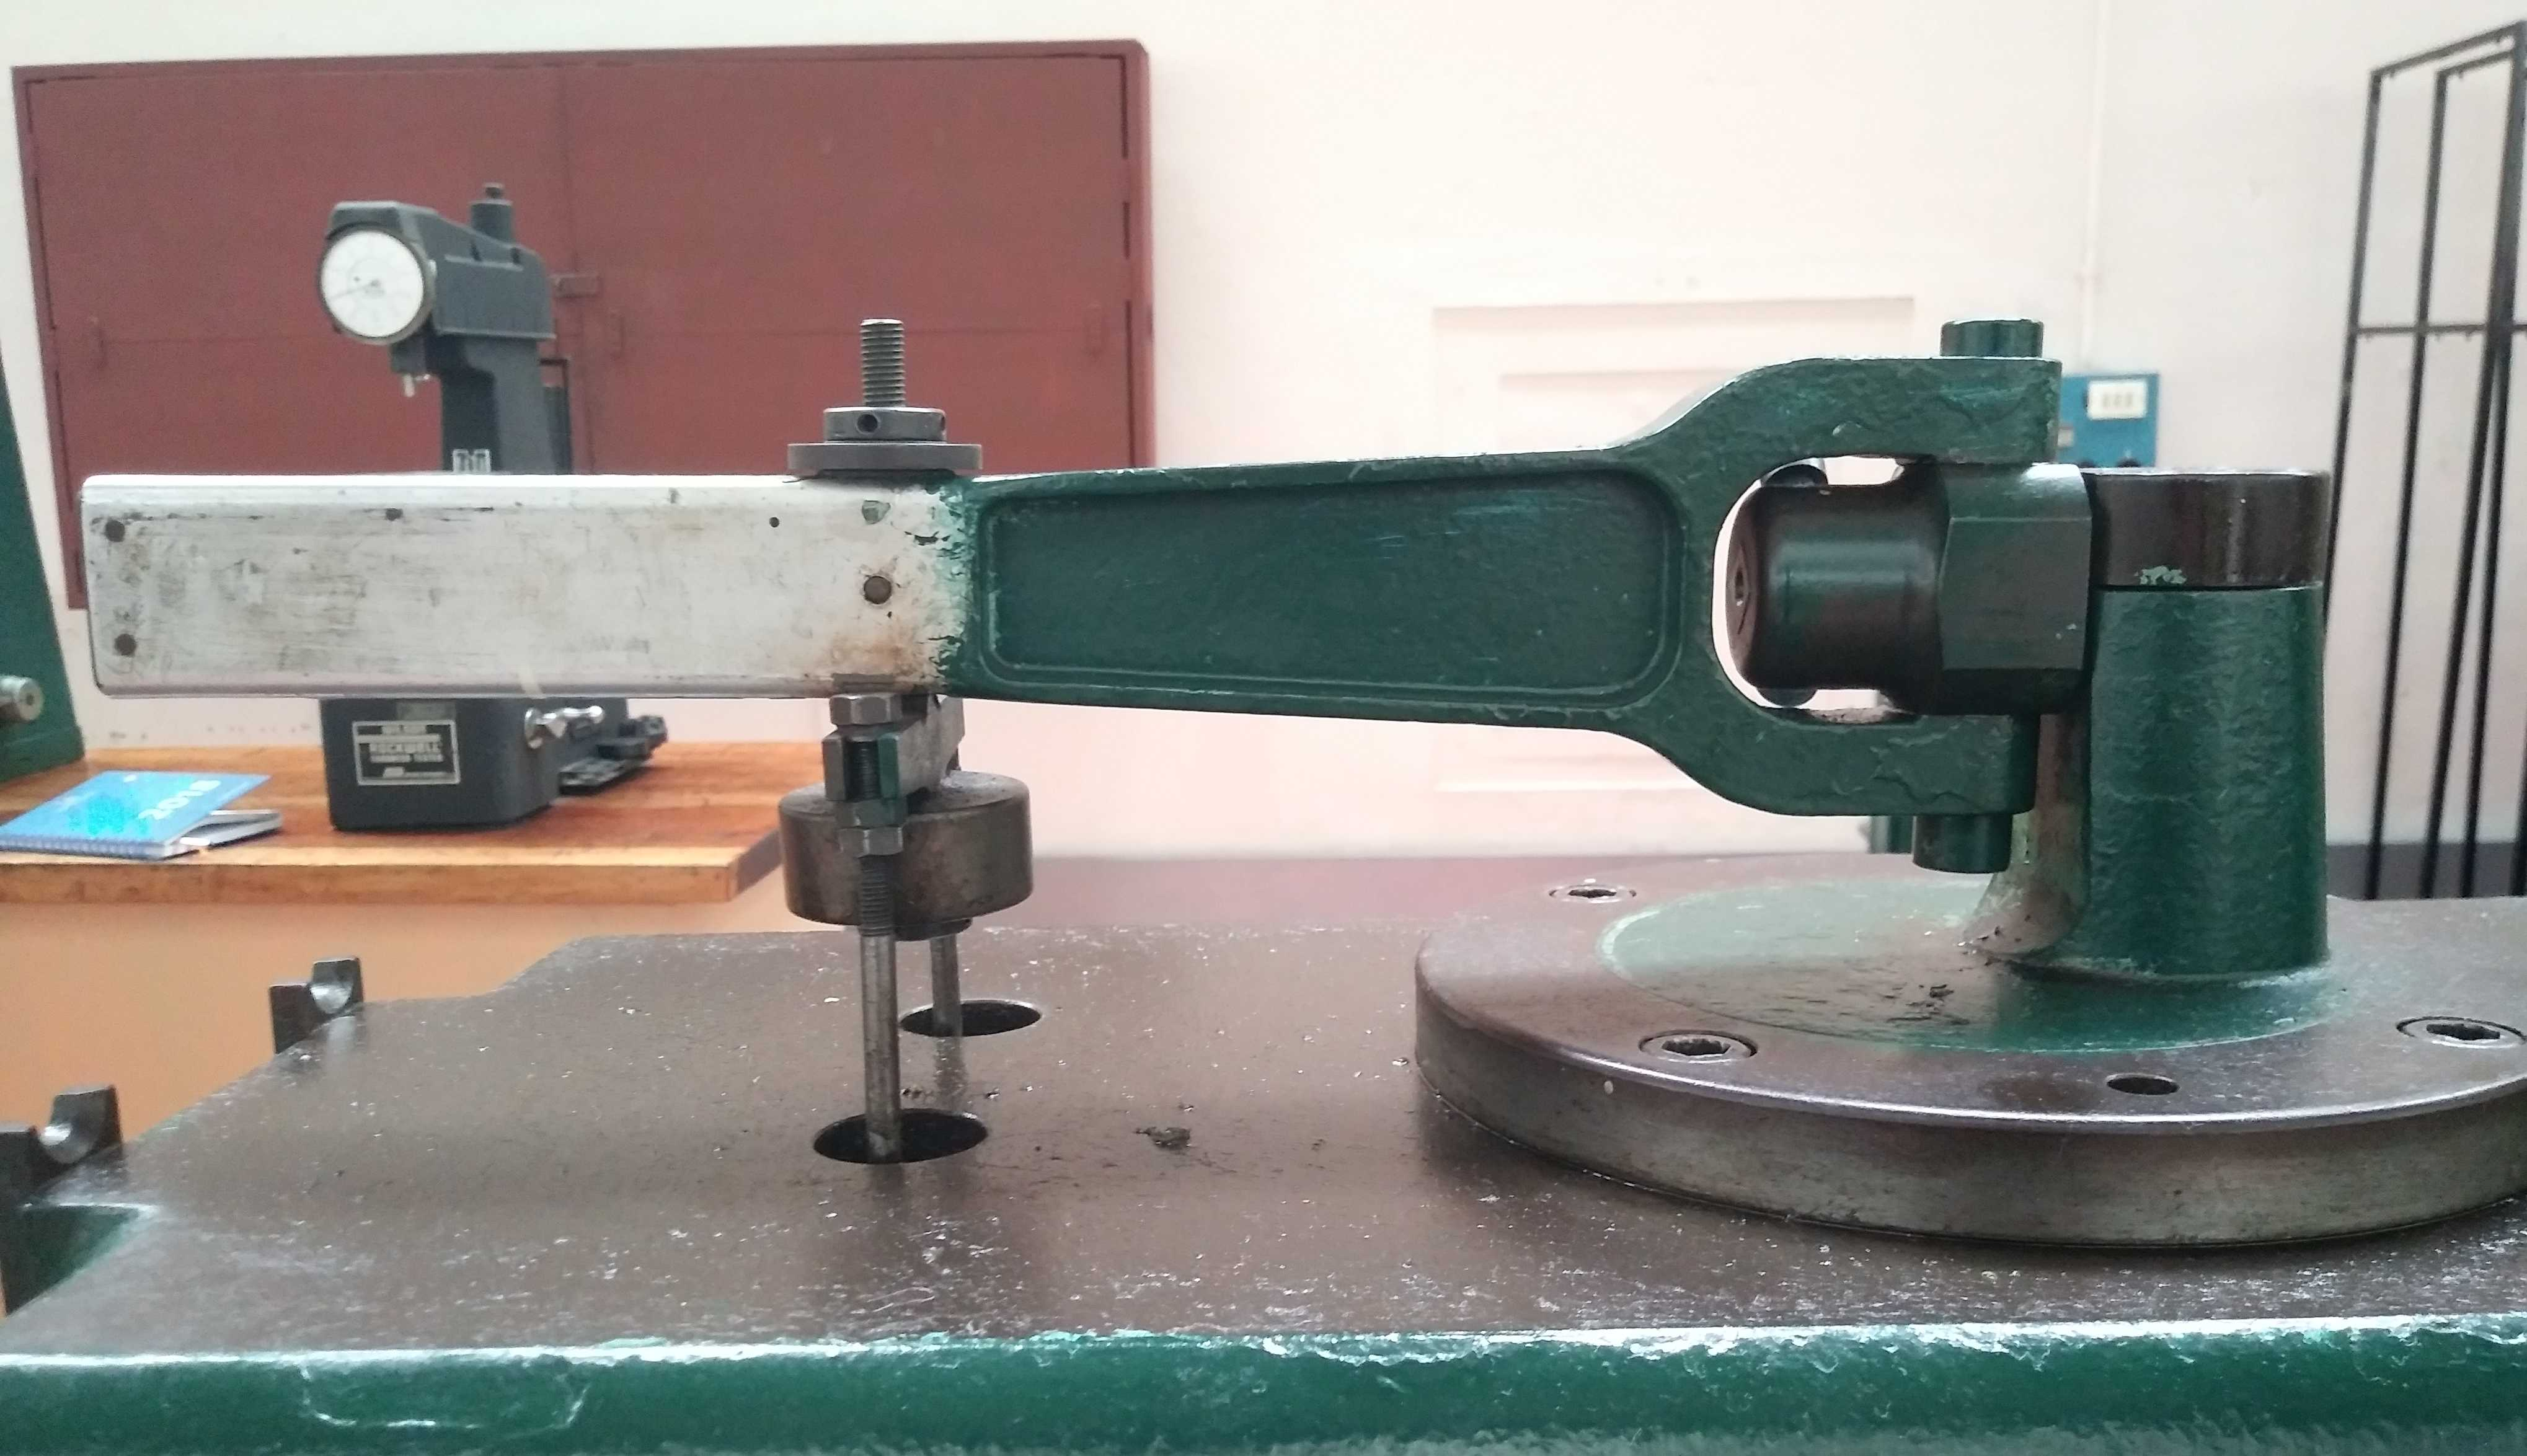
\includegraphics[width=0.9\linewidth]{Imagenes/brazo_carga.jpg}
\caption{Brazo de carga junto a su mordaza y la mordaza empotrada a la derecha.}
\label{fig:brazo_carga}
\end{figure}

La transmisión de la carga entre el disco desbalanceado y el brazo de carga se da a través de dos barras de acero redondas, uno a cada lado del disco, de diámetro 6,2 mm y largo de 169 mm.

\subparagraph{Disco desbalanceado.}
En base a las características visuales y auditivas del disco, se cree que está construido en alguna aleación de aluminio. Su radio $R_d =$ 112 mm y espesor de 6,4 mm. 

La masa de cada contrapeso, medidos en el laboratorio de metalúrgica con pesas blablabla.
\begin{table}[H]
\centering
\begin{tabular}{@{}cc@{}}
\toprule
Contrapeso & Masa {[}g{]} \\ \midrule
1          & 0,7582       \\
2          & 2,2969       \\
3          & 6,8541       \\
4          & 20,5979      \\
5          & 30,9199      \\ \bottomrule
\end{tabular}
\caption{Masa de cada contrapeso utilizado}
\label{tab:masa_contrapesos}
\end{table}

Por otra parte, no fue posible medir directamente la masa del disco al no poder desarmarlo ni separarlo de su eje. Por lo tanto, se midió de la flecha de la viga en voladizo producida por la masa del disco, la polea, el sistema de sujeción y las barras de acero, se pudo obtener la masa aproximada del disco. Sin embargo, si bien se restó la fuerza producida por la masa de las barras, se incluyó en el cálculo el resto de los elementos acompañantes del disco en la masa obtenida.

\subparagraph{Probeta.} La probeta utilizada actualmente para el ensayo de fatiga es de acero AISI 1020. Su geometría, como se aprecia en la figura REF, consiste en una pequeña viga de largo 3\nicefrac{1}{2}'', de sección cuadrada en sus extremos y una entalladura en el medio de sección circular, de lado \nicefrac{1}{2}'' de lado y 0,3'' de diámetro respectivamente.
 
\section{Diseño de estructura}
El proceso de diseñar la estructura hasta su resultado final pasó por distintas etapas. Esto por el proceso de aprendizaje y comprensión de la norma de calculo de madera NCh 1198, como también por la restricción y disponibilidad de materiales, tecnología o medidas acorde a las necesidades. El diseño presentado en este trabajo se muestra en la figura REF, hecho principalmente de madera, junto a elementos de acero. El objetivo de esta estructura es fijar y soportar la máquina de fatiga tanto en reposo como en operación, buscando como características su durabilidad, lo modular de las piezas y la opción de modificarla en el futuro.

\textcolor{red}{imagen de vista en perspectiva}

La metodología de su diseño, se separará en las distintas etapas que se realizó y los requerimientos que surgieron a partir de estas. Finalmente, se realizó una simulación estática y modal para comparar los cálculos realizados y conocer su frecuencia natural, respectivamente.
\subsection{Diseño en acero}
La estructura se diseño para que la conexión con la máquina de fatiga fuera a través de pletinas de acero, utilizando los pernos existentes. Las pletinas, a su vez , están conectadas mediante pernos a las vigas principales de madera de cada extremo. Para llevar acabo los cálculo, se hará como suposición que cada pletina esta con un empotramiento en cada extremo, con dos cargas distribuidas. La primera de ellas es el apoyo de la maquina sobre la pletina y, la segunda, el peso propio del acero. Por lo tanto, la figura REF muestra el diagrama de las cargas que actúan y las distancias a utilizar. 

\textcolor{red}{Diagrama de cargas}

Por otro lado, al no conocerse la distribución de masa de la maquina de fatiga, se considerará la carga distribuida en cada pletina como:
\begin{equation}
	 q_{maq} = \frac{0,75\cdot m_{maq}}{c} = 384,62 \; [\text{kg/m}]
\end{equation}
Donde $m_{maq}$ es la masa estimada en \ref{eq:masa_maquina}, multiplicada por 0,75 como factor de seguridad por la distribución irregular de peso de la máquina. Para obtener el esfuerzo máximo flector es necesario conocer la geometría de la viga, motivo por la cual se iteró entre las distintas opciones disponibles en el mercado de pletinas o barras planas de acero. Por razones estipuladas en la norma NCh 1198, la conexión entre la pletina de acero y la viga principal de madera se debe realizar con un mínimo de dos pernos, por lo tanto, se escogió el ancho máximo del mercad. Así, la tabla \ref{tab:dimycar_pletina} muestra las dimensiones de la pletina escogida.
\begin{table}[h]
\centering
\begin{tabular}{@{}ll@{}}
\toprule
Características pletina			       			& Valor        \\ \midrule
Espesor ($h_p$) {[}mm{]}              			& 8            \\
Ancho ($b_p$) {[}mm{]}               		    & 100          \\
Material    		                		    & A270ES	   \\
Carga distribuida ($q_{ac}$) {[}kg/m{]}		    & 6,28         \\ \bottomrule
\end{tabular}
\caption{Dimensiones y características de la viga de acero}
\label{tab:dimycar_pletina}
\end{table}

Por ende, el cálculo de la reacción en sus apoyos, el momento y esfuerzo flector máximo queda expresado por las ecuaciones \ref{eq:reaccion_acero}, \ref{eq:mtofleca_acero} y \ref{eq:esfmax_acero}, respectivamente. Estas fueron calculadas respecto al punto $A$ (o $B$, por simetría), donde se encuentra el momento flector máximo.

\begin{subequations}
	\begin{gather}
		R_A = g\left(\frac{m_{maq}}{2} + \frac{q_{ac}L}{2}\right) \label{eq:reaccion_acero}\\ 
		M_A = \left(\frac{gcq_{maq}}{24L}\right) \left(3L^2 - 4c^2 + \frac{6bc^2}{L} - \frac{3c^3}{L}\right) + \left(\frac{gq_{ac}L^2}{12}\right) \label{eq:mtofleca_acero} \\
		\sigma_{max,pl} = \frac{M_A \cdot h_p}{2I_{pl}} \label{eq:esfmax_acero}
	\end{gather}
\end{subequations}

Así, los valores obtenidos son:
\begin{itemize}
	\item $R_A = 754,85$ [N]
	\item $M_A = 100,97$ [Nm]
	\item $I_{pl} = 4266,6$ [mm$^4$]
	\item $\sigma_{max} = 94,66$ [MPa]
\end{itemize}

Con relación a la cargas fluctuantes que recibirán las pletinas como parte del funcionamiento de la máquina, se considerará la carga mayor que es capaz de producir la máquina de todas sus configuraciones, de acuerdo a lo que se obtenga por medio del modelo que se expondrá en la sección \ref{sec:mod_sist}. Esta carga alternante sobre la pletina, $F_{a,pl}$, se considerará igual a la mitad de la carga máxima posible producida por el disco desbalanceado. Por lo tanto, considerando la configuración utilizada en las cargas estáticas, la carga distribuida alternante será $q_{a,pl} = F_{a,pl}/c$ y el momento flector máximo en el punto $A$ es la primera expresión de la ecuación \ref{eq:mtofleca_acero} y el esfuerzo sobre el mismo punto igual a la expresión \ref{eq:esfmax_acero}, quedando:
\begin{gather}
	M_{a,pl,A} = \left(\frac{cq_{a,pl}}{24L}\right) \left(3L^2 - 4c^2 + \frac{6bc^2}{L} - \frac{3c^3}{L}\right)\\
	\sigma_{a,A} = \frac{M_{a,pl,A} \cdot h_p}{2I_{pl}}
\end{gather}

Para obtener el factor de seguridad, se utilizará la ecuación de Goodman modificada (\ref{eq:good_mod}). Para esto, el límite de resistencia a la fatiga de un acero se puede estimar como $S_e = 0,5S_{ut}$ cuando el esfuerzo último es menor a 1400 MPa REFERNCIA. Como el material utilizado es un acero A270ES, entonces su equivalente en la antigua nomenclatura chilena de acero es A42-27ES REFERENCIA, donde el esfuerzo último del material es $S_{ut} =$420 MPa, por lo tanto, $S_e = 210$ MPa. También, el esfuerzo medio será igual al esfuerzo estático calculado anteriormente, donde, $S_m = \sigma_{max,pl}$. Así, el factor de seguridad es:
\begin{equation}
	FS = \left(\frac{S_e\cdot S_{ut}}{S_a\cdot S_{ut} + S_m\cdot S_e}\right)
\end{equation}


\subsection{Diseño en madera}
La elección de la madera como elemento principal de construcción se debió por su capacidad de disipar las vibraciones y la relación entre su resistencia y el peso, volviendo la estructura más liviana y útil para las necesidades. Para realizar los cálculos de la madera y sus uniones, se utilizó la norma \textbf{NCh 1198 Of. 91 -- Madera: Construcciones en madera -- Cálculo}, mostrada en el anexo \ref{ch:anexo_a}. Las dimensiones del diseño de la estructura se realizaron considerando dejar el espacio necesario para la operación de la máquina, conservando la altura actual de 900 [mm]. Si bien en el presente trabajo se expondrán los cálculos de una especia maderera y sus respectivas dimensiones, se realizaron cálculos con otras especies y en otros formatos para añadir flexibilidad al diseño propuesto. Las maderas consideradas en el trabajo son el pino Oregón, pino Radiata y la línea de pino radiata encolado Hilam de Arauco. Los resultados mostrados en la sección siguiente son los obtenidos al escoger el pino Oregón en formato de 110x110 [mm]. Los valores de las tensiones admisibles para distintas especies madereras se obtienen de la tabla 4 de la sección 6.2 de la NCh 1198, sin embargo, para la madera laminada encolada se encuentran en la norma NCh 2165. Finalmente, para la sección de diseño en madera se utilizará la nomenclatura utilizada por la norma NCh 1198, para evitar confusiones al momento de consultar el anexo o la norma misma.

\textcolor{red}{añadir tabla con las dimensiones de la madera}

\subsection{Cálculo de cargas en estructura de madera}
Para identificar las distintas partes de madera en la estructura, se utilizará la figura REF como referencia. Tanto las vigas A, C, D y el pilar B, están diseñados de la misma madera y formato. En el anexo REF se pueden apreciar los planos del diseño de la estructura propuesta y sus uniones.

\textcolor{red}{añadir imagen de vigas A, B, C y D}

Como se nombró anteriormente, la madera utilizada será pino oregón, el cual bajo las consideraciones de la tabla \ref{tab:tabla3_1198} se trabajará como madera seca tanto en construcción como en servicio al estar en un ambiente cerrado sin calefacción, como se señala en la sección \ref{sec:contenido_humedad} de contenido de humedad. Los valores de densidad, tanto anhidra como normal, se pueden obtener del Anexo E de la norma. A partir de este anexo, la tabla \ref{tab:densidad_oregon} muestra los valores del pino oregón.

\begin{table}[h]
\centering
\resizebox{\textwidth}{!}{%
\begin{tabular}{@{}ccccc@{}}
\toprule
\multirow{2}{*}{\begin{tabular}[c]{@{}c@{}}Especie \\ maderera\end{tabular}} & \multicolumn{2}{c}{Densidad anhidra (kg/m$^3$)}                                                                                                & \multicolumn{2}{c}{Densidad normal (kg/m$^3$)}                                                                                                     \\ \cmidrule(l){2-5} 
                                                                             & \begin{tabular}[c]{@{}c@{}}Valor medio \\ $\rho_o$\end{tabular} & \begin{tabular}[c]{@{}c@{}}Valor característico\\ $\rho_{o,k}\,^{\dagger}$\end{tabular} & \begin{tabular}[c]{@{}c@{}}Vallor medio \\ $\rho_{12}$\end{tabular} & \begin{tabular}[c]{@{}c@{}}Valor caracerístico\\ $\rho_{12,k}\,^{\dagger}$\end{tabular} \\ \midrule
Pino oregón                                                                  & 410                                                             & 326                                                                          & 441                                                                 & 350                                                                          \\ \bottomrule
\end{tabular}%
}
\caption{Valores de la densidad normal y anhidra del pino oregón. $^{\dagger}$: Definido con el percentil 5\% de exclusión.}
\label{tab:densidad_oregon}
\end{table}

\subparagraph{Tensiones admisibles y módulo de elasticidad del pino oregón.}
Para la determinación de estos valores es necesario catalogar el grado de calidad, si corresponde a madera verde o seca y la clasificación de la madera del pino oregón. El agrupamiento de las maderas crecidas en Chile se encuentran en el anexo A de la norma NCh 1198, según la cual el pino oregón se clasifica en el grupo ES 5 para madera seca y se asumirá un grado estructural N$^{\circ}$ 4. Con esta información, a través de la tabla 6 de la norma, obtenemos que la clase estructural es F8. Con esto, la tabla 4 y 5 entrega la información de las tensiones admisibles y el módulo de elasticidad. Así, la tabla REF los valores del pino oregón utilizado en este trabajo.

\begin{table}[h]
\centering
\resizebox{\textwidth}{!}{%
\begin{tabular}{@{}ccccccc@{}}
\toprule
\begin{tabular}[c]{@{}c@{}}Clase\\ Estructural\end{tabular} & \begin{tabular}[c]{@{}c@{}}Flexión\\ $F_f$\end{tabular} & \begin{tabular}[c]{@{}c@{}}Compresión\\ Paralela $F_{cp}$\end{tabular} & \begin{tabular}[c]{@{}c@{}}Compresión\\ Normal $F_{cn}$\end{tabular} & \begin{tabular}[c]{@{}c@{}}Tracción \\ Paralela $F_{tp}$\end{tabular} & \begin{tabular}[c]{@{}c@{}}Cizalle\\ $F_{cz}$\end{tabular} & \begin{tabular}[c]{@{}c@{}}Módulo de\\ elasticidad en\\ flexión $E_f$\end{tabular} \\ \midrule
F8                                                          & 8,6 (MPa)                                               & 6,6 (MPa)                                                              & 4,1 (MPa)                                                            & 5,2 (MPa)                                                             & 0,86 (MPa)                                                 & 6,9 (GPa)                                                                          \\ \bottomrule
\end{tabular}%
}
\caption{Tensiones admisibles y módulo de elasticidad en flexión para madera de pino oregón según su clase estructural.}
\label{tab:tadm_oregon}
\end{table}

\subparagraph{Factores de modificación.}
Dada las condiciones en las que trabajará la madera, se deben calcular tres factores de modificación que afectan de manera global a la madera, sin embargo el factor de modificación por trabajo conjunto, $K_C$, no se considera en este caso. La modificación por contenido de humedad se calcula con un factor $\Delta R$ y por la diferencia entre la humedad de la madera y una humedad del 12\%, $\Delta H$. Considerando una humedad de la madera del 15\%, entonces los valores de $K_H$ para cada solicitación son los siguintes se muestran en la tabla \ref{tab:kh_oregon}.
\begin{table}[h]
\centering
\resizebox{\textwidth}{!}{%
\begin{tabular}{ccccccc}
\hline
\begin{tabular}[c]{@{}c@{}}Factor de \\ modificación\\ por humedad\end{tabular} & \begin{tabular}[c]{@{}c@{}}Flexión\\ $F_f$\end{tabular} & \begin{tabular}[c]{@{}c@{}}Compresión\\ Paralela $F_{cp}$\end{tabular} & \begin{tabular}[c]{@{}c@{}}Compresión\\ Normal $F_{cn}$\end{tabular} & \begin{tabular}[c]{@{}c@{}}Tracción \\ Paralela $F_{tp}$\end{tabular} & \begin{tabular}[c]{@{}c@{}}Cizalle\\ $F_{cz}$\end{tabular} & \begin{tabular}[c]{@{}c@{}}Módulo de\\ elasticidad en\\ flexión $E_f$\end{tabular} \\ \hline
$K_H$                                                                           & 0,999385                                                & 0,999385                                                               & 0,999385                                                             & 0,99952                                                               & 0,999199                                                   & 0,999556                                                                           \\ \hline
\end{tabular}%
}
\caption{Valores del factor de modificación para el pino oregón.}
\label{tab:kh_oregon}
\end{table}

Por otro lado, el factor de modificación por duración, $K_D$, se aplica a través de la ecuación \ref{eq:k_d}, donde la duración de la carga $t$ se aplica en segundos. También, la norma incluye el gráfico de $K_D$ siendo una opción para su cálculo. Los valores admisibles que se señalan en la norma corresponden a una vida útil de 10 años de duración, sin embargo, para una vida útil indefinida el valor de $K_D$ corresponde a 0,9. Este factor de modificación no afecta al módulo de elasticidad ni a la tensión admisible de compresión normal.
\begin{equation} \label{eq:k_d}
	K_D = \frac{1,747}{t^{0,0464}} + 0,295
\end{equation}

\subsubsection{Viga principal, A}
Es la viga que soporta la carga de las pletinas que sostienen a la máquina y a su vez descansa la carga en los pilares B. Para realizar los cálculos de esfuerzo se consideró un doble empotramiento en cada extremo, con tres cargas distribuidas que representan la carga de las pletinas de acero, $q_{pl}$, las cuales se determinarán según la ecuación \ref{eq:q_pl}, y el peso propio de la madera.
\begin{equation}\label{eq:q_pl}
	q_{pl} = \frac{q_{maq}\,c + q_{ac}\,L}{2b_p}
\end{equation}
El diagrama y la distribución de la carga se puede apreciar en la figura REF. Por otro lado, el esfuerzo máximo se presenta en los extremos de la viga. Las ecuaciones \ref{eq:reac_vigappal} y \ref{eq:mto_vigappal}, muestran la obtención de las reacciones y del momento flector máximo.
\begin{subequations}
\begin{gather}
	R_0 = g \left( q_{pl}\cdot b_p + \frac{L\cdot q_{mad}}{2}\right) \label{eq:reac_vigappal}\\
	M_0 = \left(\frac{q_{pl}\cdot g\cdot b_p}{L^2}\right) \left(l_2 l_6^2 + l_6 l_2^2 - \frac{b_p^2}{12}\left( l_6 + l_2\right) \right) + \frac{R_0\cdot L}{6} \label{eq:mto_vigappal} 
\end{gather}
\end{subequations}
Donde los valores obtenidos son:
\begin{itemize}
	\item $R_0 = Q = 795$ [N]
	\item $M_0 = M_{max} = 122,26$ [Nm]
\end{itemize}
Así, la tensión de trabajo $f_f$ se calcula según la ecuación \ref{eq:f_f}, obteniendose el valor:
\begin{equation}
	f_f = 0,551 \quad \text{(MPa)}
\end{equation}
De este modo, la tensión de diseño en la zona flexo-traccionada y flexo-comprimida que se calcula a partir de \ref{eq:ft_dis} y \ref{eq:fv_dis}, respectivamente. Para la zona flexo-traccionada se debe calcular el factor de modificación por altura y para la flexo-traccionada el factor de modificación por volcamiento. El primero se obtiene con la ecuación \ref{eq:khf}, obteniendose el valor de $K_{hf} = 0,916$. Para el factor de volcamiento, se deben verificar el caso que corresponde como se señala en el anexo \ref{ch:anexo_a}, el cual da un valor de $K_v=1$. Por lo tanto, el valor de $F_{ft,dis}$ y $F_{fv,dis}$ son:
\begin{subequations}
\begin{gather}
	F_{ft,dis} = 7,08 \quad \text{(MPa)}\\
	F_{fv,dis} = 7,74 \quad \text{(MPa)} 
\end{gather}
\end{subequations}
Por otro lado, la tensión de trabajo en cizalle se obtiene a partir de la ecuación \ref{eq:f_cz} y la de diseño en cizalle por \ref{eq:cz_dis}. Dado que $K_r=1$ al no haber rebajo de la viga, entonces el valor obtenido para ambas tensiones son:
\begin{gather}
	f_{cz} = 0,098 \quad \text{(MPa)}\\
	F_{cz,dis} = 0,774 \quad \text{(MPa)}
\end{gather}
Finalmente, los valores de factor de seguridad (FS) para cada uno de las tensiones calculadas son los siguientes:
\begin{subequations}
\begin{gather}
	FS_{ft} = 12,85\\
	FS_{fv} = 14,03\\
	FS_{cz} = 7,85
\end{gather}
\end{subequations}

\subsubsection{Pilar de apoyo, B}
El pilar B representa los cuatro apoyos de la estructura, recibiendo la carga de la máquina y su operación desde la viga principal y transmitiendola hasta el piso. Por la disposición del cuartón, estará sometido a compresión paralela (\ref{sec:cp}). Al igual que en la viga principal, se debe calcular la tensión de trabajo ($f_{cp}$) y la tensión de diseño en compresión paralela ($F_{cp,dis}$). Al ser el mismo formato y especie maderera de la viga principal, su área transversal sigue siendo de 110x110 mm, mientras que el largo del pilar ($L_v$) corresponde a 790 mm.

Para el primero, se obtiene a través de la ecuación \ref{eq:f_cp}, donde la carga $N$ será igual a la reacción obtenida en \ref{eq:reac_vigappal}. Así, su valor es:

\textcolor{red}{Corregir con área modificada por pernos}
\begin{equation}
	f_{cp} = 0,0657 \quad \text{(MPa)} 
\end{equation}
Para el segundo, el cálculo de la tensión de diseño dependerá de la inestabilidad lateral dado por la esbeltez $\lambda$. La longitud efectiva de pandeo se obtiene a través de la tabla 18 de la norma, de la cual se escogerá la configuración de apoyo con impedimento de giros y desplazamiento por un extremo y, para el otro lado, impedimento de giro con libertad de desplazamiento, es decir, $l_p/L_v = 1,5$. De esta forma, los valores obtenidos son:
\begin{gather*}
	l_p = 1,5\cdot L_v = 1,185 \: \text{(m)}\\
	i = \sqrt{\frac{I}{A}} = \sqrt{\frac{0,11^4}{12\cdot 0,11^2}} = 0,032 \: \text{(m)}\\
	\lambda = \frac{l_p}{i} = 37,32 \: \text{(-)}
\end{gather*}
Como $\lambda > 5$, entonces la tensión de trabajo de compresión paralela se debe calcular según \ref{eq:cp_dislambda} y se debe evaluar el factor de modificación por esbeltez $K_{\lambda}$ a partir de \ref{eq:k_lambda}. El coeficiente de proporcionalidad para una madera de grado n$^{\circ}$ 4 es $c = 0,8$ y el módulo de elástico de diseño es $E_{dis} = 6206,2\: \text{(MPa)}$. Por otro lado, la tensión de diseño $F_{cp,dis}$ se obtiene según \ref{eq:cp_dis} y los factores de modificación $K_D$ y $K_H$.
\begin{equation}
	F_{cp,dis} = 5,936 \: \text{(MPa)}
\end{equation}
Con esto, los valores de las constantes y el factor de modificación serán $A = 2,852\;$ (-), $B = 3,754\;$ (-) y $K_{\lambda} = 0,759\:$ (-). Así, el factor de modificación final $F_{cp,\lambda, dis}$ será:
\begin{equation}
	F_{cp,\lambda, dis} = 4,506 \: \text{(MPa)}
\end{equation}
Finalmente, el factor de seguridad con esta configuración es:
\begin{equation}
	FS_{cp,\lambda} = 68,6\: \text{(-)}
\end{equation}

\subsubsection{Viga transversal, C}
Para esta viga se realizará el mismo procedimiento que para la viga A, sin embargo, las solicitaciones son menores y la única carga a la que está sometida es la de su propio peso. Las dimensiones nominales de la tabla son 1x8'' cepillada, es decir, según las tablas de valores \ref{tab:anchodim} y \ref{tab:espdim} son de 19x185 mm y su largo es de 800 milímetro. La carga distribuida de su peso es de $q_{tabla}=1,5$ [kg/m].

Debido a lo bajo de las solicitudes, las tensiones de trabajo en flexión son:
\begin{equation}
	f_f = 3,804 \: \text{(kPa)} 
\end{equation}
Por otro lado, por las dimensiones de la madera usada, el factor de modificación por altura y volcamiento son los siguientes:
\begin{gather*}
	K_{hf} = 0,864\: \text{(-)}\\
	K_{v} = 0,586\: \text{(-)}
\end{gather*}
El cálculo de $K_v$ se realiza con la ecuación \ref{eq:k_v}, porque la esbeltez del límite elástico es menor a la esbeltez de volcamiento.
\begin{gather*}
	\lambda_v = 23,38 \: \text{(-)}\\
	\lambda_{vo} = 21,95 \: \text{(-)}
\end{gather*}
Así, la tensión de diseño en flexión de esta viga es de:
\begin{equation}
	F_f = 3,9235 \: \text{(MPa)}
\end{equation}
\subsection{Uniones}
Las uniones en madera se deben diseñar siguiendo las indicaciones establecidas en la sección 10 de la norma NCh1198, uniones en la madera estructural. Esta considera la condición de la madera en operación, el tipo de unión, la dirección de la solicitación repecto a la dirección de la fibra, el número de elementos de unión, el distanciamiento entre los elementos de unión y el tipo de cizalle. Para el diseño de la estructura se utilizaron tres elementos de unión distintos: tirafondos, pernos \textcolor{red}{ y, en menor medida, clavos.}

\subsubsection{Acero - madera}
Para la unión entre la pletina de acero y la viga principal de madera, se utilizaron dos pernos de grado 2 de 4 \nicefrac{1}{2}'' de largo y  $3/8''$ de diámetro. Como se explica en la sección \ref{sec:union_perno} el mínimo de pernos por unión debe ser dos, con la excepción de que el único perno no esté solicitado en un porcentaje superior al 50\% de su capacidad de diseño. La unión está compuesta por la pletina de acero, seguido por la viga de madera con la dirección de sus fibras normal a las solicitaciones y nuevamente una placa de acero. Finalmente, para el cálculo de la capacidad de carga admisible y tensión admisible de aplastamiento nominal, se recurrirá a las ecuaciones \ref{eq:padm_ad} y \ref{eq:f_ap}, respectivamente. 

Para calcular la capacidad de carga admisible, $P_{ad}$, se utilizaron las indicaciones para cizalle simple, las cuales indican que se determina como el menor valor de la mitad de la carga admisible de cizalle doble entre una pieza central de espesor igual a la pieza más grande y una pieza central igual al dobleasí  del espesor de la pieza más delgada. Para este diseño el valor menor consiste en considerar el espesor central ficticio $e*$ como dos veces el espesor menor, es decir, el espesor lateral $e_l$, así el valor de esbeltez del perno es:  
\begin{equation*}
	\lambda_u = \frac{2\cdot e*}{D} = \frac{2\cdot 8\, \text{mm}}{9,525\, \text{mm}} = 1,679\: \text{(-)}
\end{equation*}
Para obtener los valores de $F_{ap}$ el valor del factor de reducción de zona elástica se obtiene a partir de la densidad anhidra de la madera (tabla \ref{tab:densidad_oregon}, siendo $\eta =$ 2,2. Por otro lado el ángulo $\theta$ es de $\pi/2$ al estar las fuerzas en dirección normal a la fibra de madera. Con esto, se obtiene:
\begin{gather}
	F_{ap} = 3,402 \: \text{(MPa)} \\
	P_{ad,simple} =\frac{P_{ad,doble}}{2} = 259,24 \: \text{(MPa)}
\end{gather}
Para terminar, se debe corroborar que se cumple la desigualdad de la ecuación \ref{eq:padm_ad}, así:
\begin{equation*}
	Z\cdot D^2 = 2131,94 \: \text{(MPa)} \geq 259,24 \: \text{(MPa)}
\end{equation*}

\subparagraph{Espaciamiento}
El espaciamiento entre los pernos se especifica en la sección \ref{sec:espaciamiento_pernos}, de las cuales se obtiene la distancia entre pernos y los bordes es:
\begin{align*}
	S_{bcn} &= 1,5 \, \text{mm} \\
	S_{bdn} &= 0,75 \, \text{mm} \\
	S_p &= 2,625 \, \text{mm}
\end{align*}


\subsubsection{Madera - Madera}
Existen distintos componentes de unión para la conexión de elementos de madera. En este trabajo se utilizó el tirafondo, perno y clavo como elementos principales de unión.  Cada uno de ellos tiene distintas características que los vuelven ventajosos en ciertas situaciones. La utilización del tirafondo se utiliza para unir la viga C con el pilar B y la viga A, por su capacidad de ``empujar'' una madera contra la otra de manera eficiente. Los pernos, por otro lado, se utilizaran para la unión de herrajes entre la viga D y el pilar B, como también en los herrajes de anclaje del pilar B con el piso. En el caso de los clavos, estos se ocupan en los  herrajes o ángulos de apoyo entre las vigas A y B, para evitar su movimiento transversal. Para estos dos últimos elementos de unión, su elección está supeditada a las recomendaciones del fabricante de los herrajes o ángulos, quienes incluyen los valores de carga en la elección de los elementos de unión. Por lo mismo, la caracterización de estos elementos se realizará en la sección de herrajes.

\subsubsection{Tirafondos}
Las indicaciones para el cálculo, espaciamiento e instalación de los tirafondos se encuentran en la sección \ref{sec:tirafondos}. Al igual que el proceso de selección de vigas de madera, se iteró con distintas dimensiones de largo y diámetro. Así el tirafondo escogido fue de $1/4$x3\nicefrac{1}{2}'', lo cual se traduce a partir del anexo M de la norma en las medidas expuestas en la tabla \ref{tab:tirafondo}.
\begin{table}[h]
\centering
\resizebox{\textwidth}{!}{%
\begin{tabular}{@{}cccccl@{}}
\toprule
\begin{tabular}[c]{@{}c@{}}Nomenclatura\\ tirafondo\end{tabular} & \begin{tabular}[c]{@{}c@{}}Diámetro Nominal \\ ($D_v$ o $D$) [mm]\end{tabular} & \begin{tabular}[c]{@{}c@{}}Diámetro de rosca\\  ($D_R$) [mm]\end{tabular} & \begin{tabular}[c]{@{}c@{}}Largo roscado\\  (R) [mm]\end{tabular} & \begin{tabular}[c]{@{}c@{}}Largo vástago\\ (V) [mm]\end{tabular} & \begin{tabular}[c]{@{}l@{}}Largo punta\\ (P) [mm]\end{tabular} \\ \midrule
$1/4$x3\nicefrac{1}{2}''                                         & 6,4                                                                            & 4,4                                                                       & 51                                                                & 38                                                               & 4,8                                                            \\ \bottomrule
\end{tabular}%
}
\caption{Dimensiones del tirafondo utilizado}
\label{tab:tirafondo}
\end{table}

Para su instalación, la norma indica que es necesario realizar perforaciones guías, las cuales están en función de sus características. Así el agujero tendrá dimensiones para la zona del vástago y otra para la zona con rosca. Para la zona del vástago, el agujero deberá tener las dimensiones del diámetro nominal $D_v$ y el largo V. Para la segunda zona, la madera de pino oregón se categoriza en el grupo B según su densidad anhidra, a partir de la tabla 38 de la norma. Con esta información el largo del agujero debe ser de R - P  y el diámetro del entre el 60\% y el 70\%.
\subparagraph{Solicitaciones de extracción lateral}
La carga admisible de extracción lateral se calcula según la ecuación \ref{eq:pel_ad}. El valor K se obtiene a partir de la tabla 39 de la norma a partir de si la madera utilizada es conífera o latifoliada y su densidad anhidra. El pino oregón es una madera conífera y, según su densidad, el valor de K es de 11,7. Así el valor obtenido es de $P_{el,ad} = 0,48$ (kN). Sin embargo, la norma establece tres condiciones que se deben cumplir para que la expresión \ref{eq:pel_ad} sea aplicable, de las cuales no se cumple que el espesor $e_L$ de la pieza lateral atravesada por el tirafondo sea igual a $3,5\cdot D$. Por esto se debe mayorar el valor de la carga admisible por factores de modificación que pueden penalizar o ayudar, dependiendo de la configuración de la unión.

\subparagraph{Factor de modificación por espesor de la pieza lateral.}
El factor se obtiene a partir de la tabla 40 de la norma, debido a que $e_L \neq 3,5\cdot D$. El valor $K_{te}=0,93$ se obtiene al ingresar a la tabla con la razón $e_L/D \approx 3$.

\subparagraph{Factor de modificación por penetración del vastago en la pieza principal.}
De manera análoga, el factor se obtiene en la tabla 41 de al norma a partir de la razón la penetración del vástago en la pieza, $P_v$ y el diámetro del tirafondo. El valor de este es $P_v/D \approx 5$, lo cual da que $K_v=1,36$

\subparagraph{Factor de modificación por diámetro.}
Por último, este factor se obtiene directamente del diámetro nominal del tirafondo, a través de la tabla 42 de la norma. El valor corresponde a $K_{tD}=0,97$.

Además de los factores de modificación expuestos, el eje del tirafondo se encuentra en dirección paralela a las fibras de la madera de la pieza principal, por lo tanto se debe multiplicar el valor de la carga admisibles por $2/3$. En conclusión, la carga admisible es igual a :
\begin{equation}
	P_{el,ad} = \frac{2}{3}\cdot K_{te}\cdot K_{tv}\cdot K_{tD} \cdot K\cdot D^2\cdot = 391,966 \: \text{(N)}
\end{equation}

\subparagraph{Solicitaciones de extracción directa}
Para el caso de la extracción directa es la ecuación \ref{eq:ped_ad} la que determina la carga admisible de tirafondos colocados con su eje normal a las fibras de la madera. Dado que este no es el caso, como se señaló en la sección de extracción lateral, la carga admisible a considerar se debe multiplicar por $3/4$. Por otra parte, el valor de la longitud crítica de penetración $l_{crit}=10\cdot D_R$ se obtuvo de la tabla 43 de la norma. Sin embargo, la longitud real de penetración de la zona roscada (R-P) es menor a la longitud crítica, por lo tanto en la ecuación se reemplaza $l_{crit}$ por $l = R-P$. Entonces el valor obtenido para la carga admisible es:
\begin{equation}
	P_{ed,ad} = 6,37 \: \text{(kN)}
\end{equation} 

\subsubsection{Herrajes y conectores}
La elección de los conectores y herrajes utilizados se baso en tres aspectos principales: la disponibilidad de los productos en la región, la compatibilidad con los elementos de madera y con las cargas que pueden resistir según el fabricante. Estos consisten en un elemento de metal, acero generalmente, que permite la unión de dos o más piezas de madera para soportar determinadas cargas. Existen en distintas geometrías y el mecanismo de conexión entre acero y madera es a través de elementos de unión mecánica, es decir, pernos, clavos y tornillos, principalmente. Para este trabajo se utilizaron tres tipos, los cuales une las vigas A y B, B y D y B con el suelo del laboratorio, todos fabricados por la marca Simpson Strong-Tie.

Para la primera unión se utilizó en el diseño un ángulo de apoyo modelo A66, donde cada brazo tiene una longitud de 6''. La unión mecánica utilizada son los clavos de \textcolor{red}{buscar dimensiones}. Como se puede apreciar en la figura REF, este ángulo busca responder a las fuerzas que son paralelas al plano horizontal.

\textcolor{red}{imagen A66}

Para la unión del pilar B y la viga D se utilizó \textcolor{red}{colocar nombre}. Este se une a través de un perno por cada brazo de \textcolor{red}{dimensiones}. Estos buscan soportar la carga provocada por el propio peso y evitar los desplazamientos horizontales. Su disposición se puede ver en la figura REF, donde se aprecia cómo se utilizan dos ángulos por conexión.

\textcolor{red}{Detalle del diseño de la mesa}

Por último, la unión entre el piso y el pilar B se escogió un ángulo de anclaje A24. Utiliza un perno de anclaje para el piso y otro normal que es adosado en el otro extremo del pilar por un segundo ángulo de anclaje, de manera similar a la unión B-D. La imagen REF muestra en detalle el diseño de la conexión.
 
\subsection{Simulaciones}
Las simulaciones de la máquina se utilizaron como apoyo y contraparte de los cálculos realizados manualmente. Éstas se realizaron en el software Inventor AutoCAD, en el ambiente ``\textit{Stress Analysis}''. A través de esto se busco confirmar que los resultados obtenidos en los cálculos estáticos se encuentran fuera de los rangos de falla y obtener las frecuencias naturales de la estructura, utilizando ``\textit{Static and Modal Analysis}'' respectivamente.

Debido a las limitantes del programa utiilzado, se debieron adaptar las propiedades mecánicas ortotrópicas de la madera, las cuales no era posible simular directamente. Para esto, se utilizaron los valores mínimos del Módulo de Young y las tensiones admisibles en sus direcciones normales y perpendiculares, buscando representar de manera segura las propiedades ortotrópicas en una configuración isotrópica.

Como condición del problema, en ambas simulaciones, los apoyos del pilar se consideraron empotrados, restringiendo cualquier grado de movimiento en su base. Además, las uniones se consideraron perfectas y sin desplazamientos.
\subsubsection{Estática}
Las condiciones...
\subsubsection{Modal}
La configuración...

\section{Modelo del sistema de vibratorio}
Luego del levantamiento de información, se busca analizar y predecir el comportamiento de la máquina en sus distintas configuraciones. Para esto se utiliza la información disponible para realizar un modelo del funcionamiento de la máquina de fatiga, en específico, de la carga aplicada a la probeta en función de la velocidad de rotación del disco y las distintas combinaciones de contrapesos. El disco se encuentra en voladizo, cuyo desequilibrio a partir de los contrapesos colocados produce una fuerza que es transmitida hacia un brazo de carga. Este, a su vez, aplica un momento de flexión sobre una probeta que está doblemente empotrada por mordazas.

Para obtener el comportamiento y la fuerza que produce el desbalanceo en el disco sobre la probeta, se modelará un sistema de dos grados de libertad para representar el movimiento de la máquina y sus componentes, realizando ciertas simplificaciones y suposiciones. Se utilizará el método de energía para resolver el sistema.

A través de esto, se pretende obtener la posición en reposo de la máquina y la deformación máxima que sufre la probeta según la combinación de contrapesos. En concreto, la posición en reposo de la máquina, en otras palabras, la deformación producto de la masa de los elementos, entregará información sobre cual es la carga media y esfuerzo medio que sufre la probeta. En cambio, la deformación máxima es la información relativa al esfuerzo alternante que se le aplica a la probeta según la configuración utilizada. Por ello, el modelo deberá partir de una posición a conveniencia en un tiempo inicial y sin fuerzas externas interviniendo. Posteriormente, una vez que se haya alcanzado la posición de equilibrio, la fuerza externa producida por el disco desbalanceado comenzará a funcionar hasta que vibre de manera estacionaria. Al respecto, al ser la fuerza dependiente de la velocidad angular del disco, se introducirá una función que llamaremos $\phi$ la cual controlará la aceleración y velocidad del disco.

\subsection{Elementos del sistema}
La imagen REF muestra todas los elementos que participan en el funcionamiento de la máquina y que afectan su comportamiento. Sin embargo, estos se llevarán a un diagrama que representará los elementos y las simplificaciones utilizadas para modelar el movimiento de la máquina, en específico, del brazo de carga.  

\textcolor{red}{Foto de la máquina abierta}

\subsection{Modelo del sistema}
\label{sec:mod_sist}
Como se señaló, para poder crear un modelo del sistema y obtener soluciones, se realizaron simplificaciones y suposiciones que permiten llegar a una solución. Así, la figura REF muestra el diagrama que se modelará con las ecuaciones de movimiento. Parte de estas simplificaciones es la exclusión de las fuerzas horizontales, en dirección de la coordenada $x$, de acuerdo a la referencia utilizada. Para esto, también es necesario quitarle los grados de libertad a la barra de transmisión de la carga y simplificar la carga producida por la rotación del disco, explicado en la sección siguiente. Por último, se asumirá que el movimiento angular del brazo de carga será lo suficientemente pequeño como linealizar la función trigonométrica del ángulo $\theta$, aproximándose los valores de $\sin(\theta) = \theta$ y $\cos(\theta)=1$.

\begin{figure}[h]
\centering
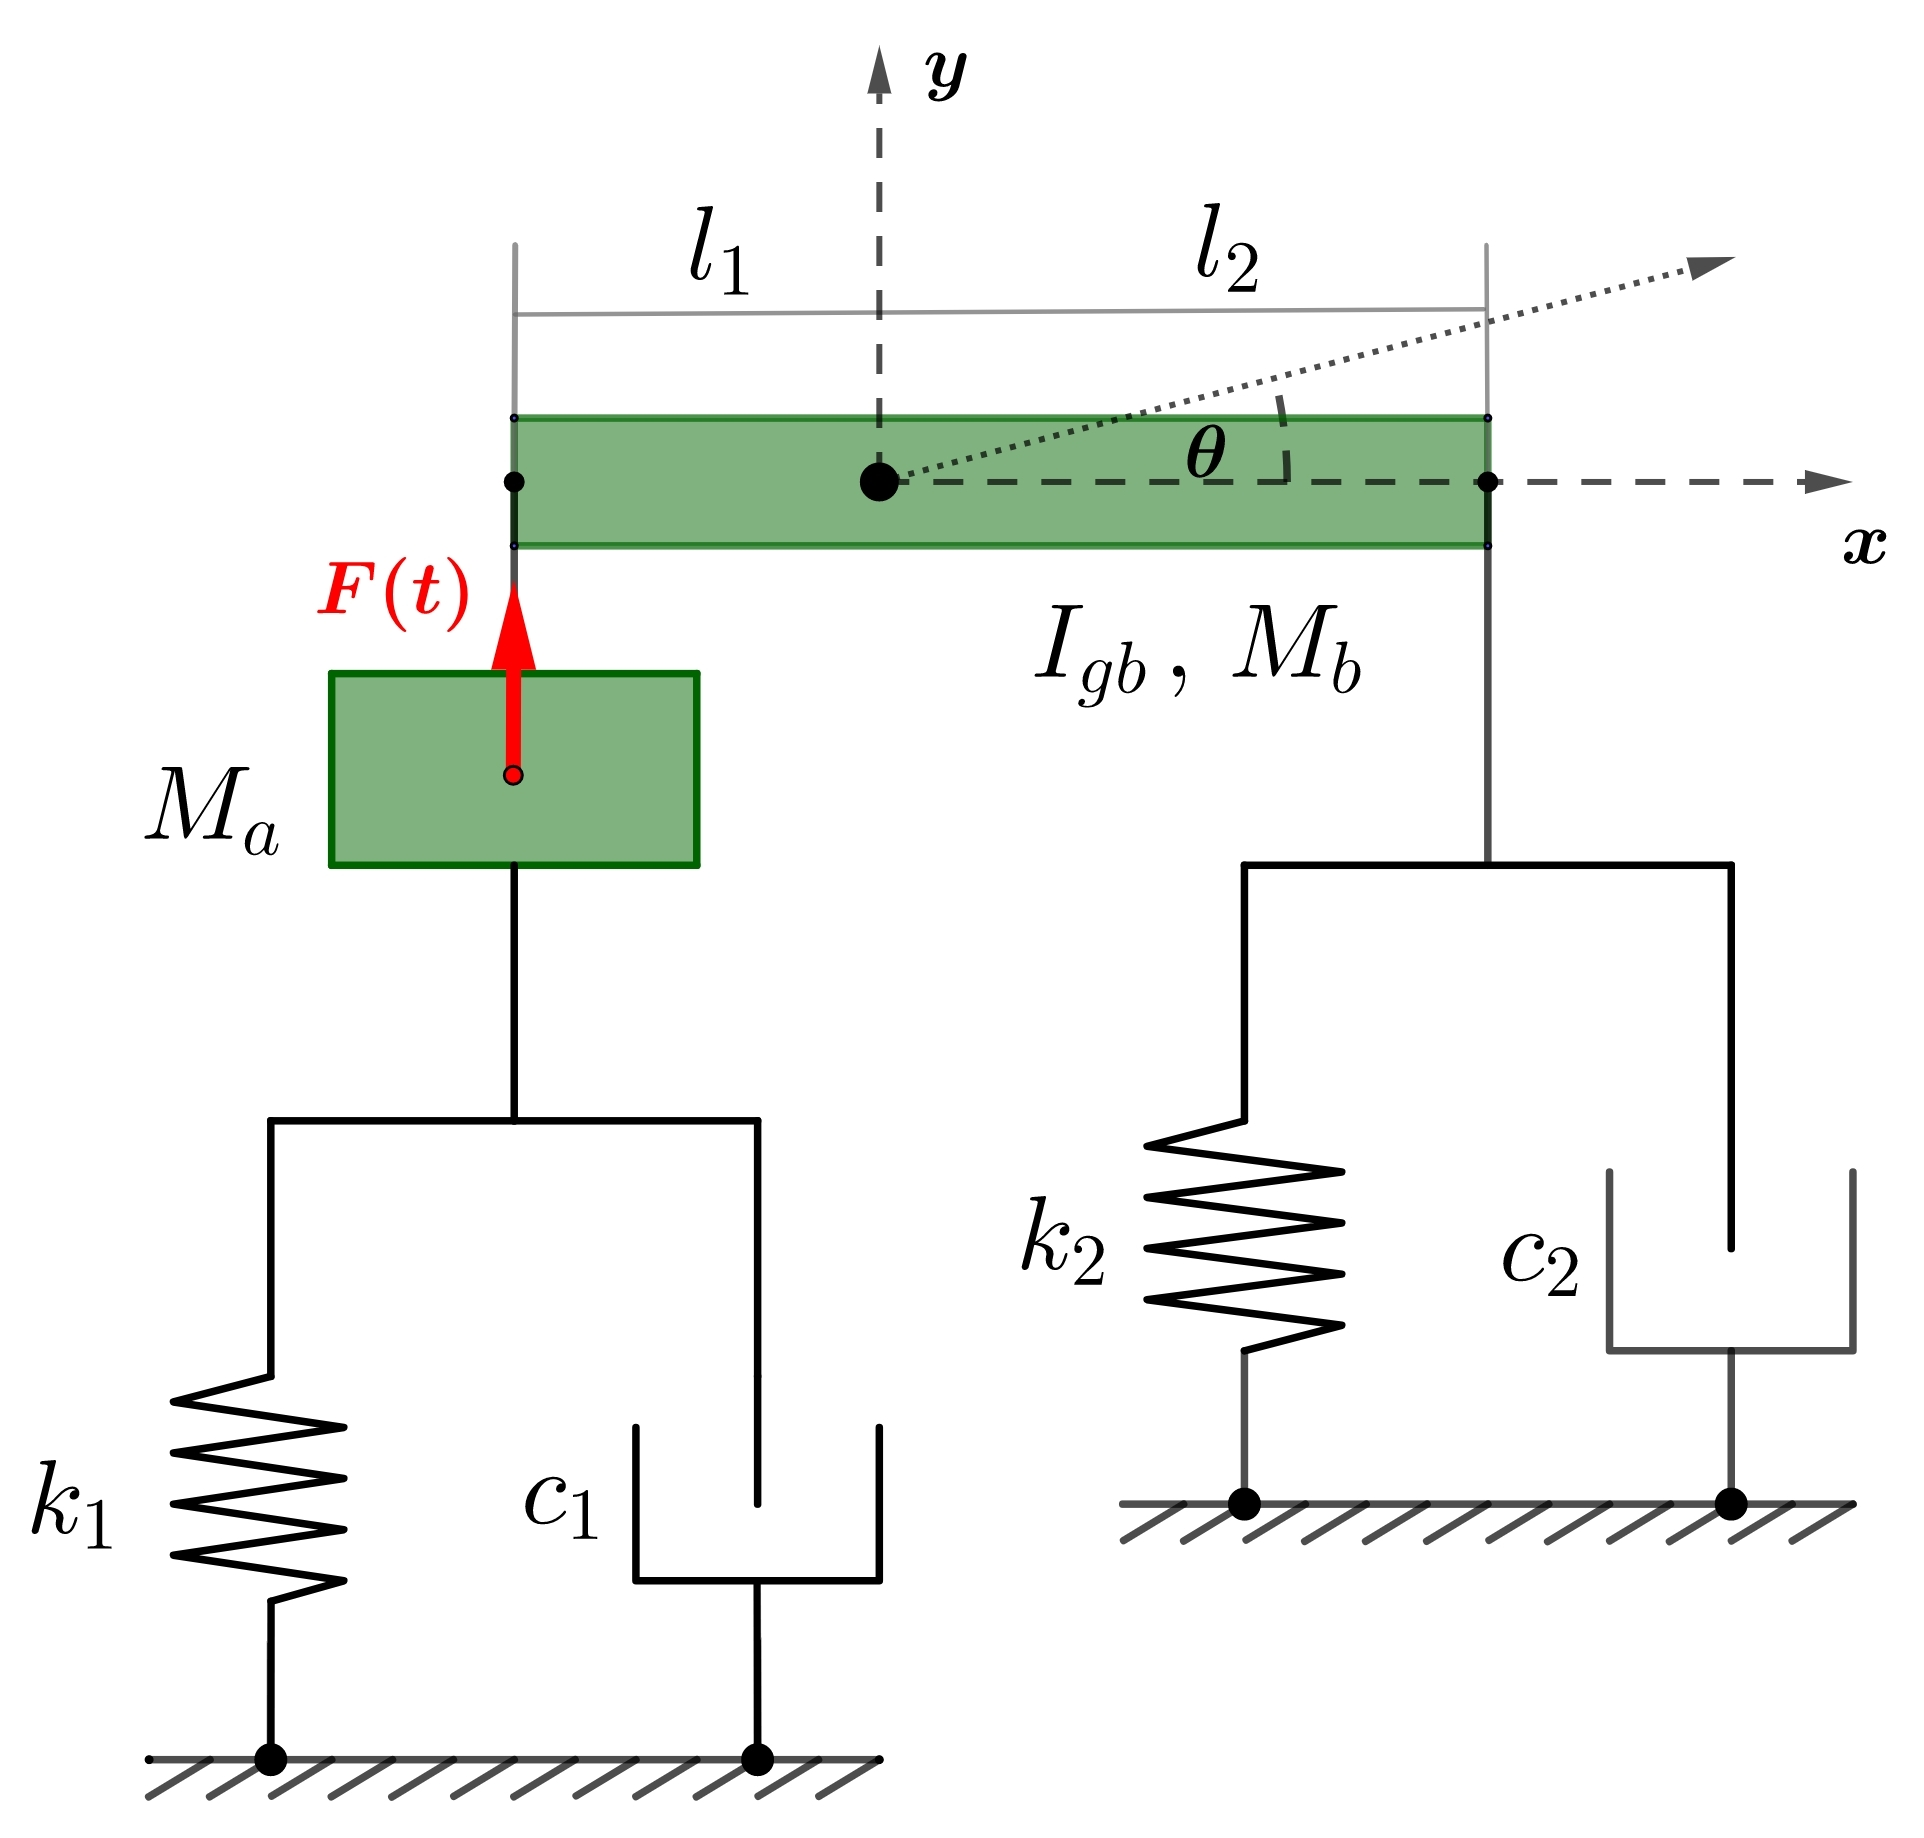
\includegraphics[scale=0.13]{Imagenes/mach_diagram.jpg}
\caption{Diagrama del modelo utilizado y el sistema de coordenadas.}
\label{fig:diag_modelo}
\end{figure}

Los sistemas de coordenadas $y(t)$ y $\theta (t)$ definen la posición y el movimiento del brazo de carga en cualquier instante $t$. Al ser independientes entre sí y no depender de ninguna restricción, es que las coordenadas generalizadas serán $q_1 = y$ y $q_2 = \theta$. A modo de conveniencia se establecerán las variables $y_1$ e $y_2$, las cuales describen el movimiento en ambos extremos del brazo.
\begin{gather}
	y_1(t) = y(t) - l_1\theta(t) \label{eq:y1}\\
	y_2(t) = y(t) + l_2\theta(t) \label{eq:y2}
\end{gather}
Cuando $y(t_0) = 0$ y $\theta(t_0) = 0$ la deformación en ambos resortes será cero, por lo tanto las variables $y_1$ e $y_2$ son equivalentes a la deformación de los resortes. La rigidez de cada resorte se denotarán como $k_1$, relativo a las barras de acero, y $k_2$, relativo a la probeta.

Por otro lado, la velocidad de las coordenadas se definirán como $\dot{y}(t)$ y $\dot{\theta}(t)$ y, de manera análoga, la aceleración como $\ddot{y}(t)$ y $\ddot{\theta}(t)$. A partir de las ecuaciones \ref{eq:y1} y \ref{eq:y2} se obtiene que:
\begin{gather}
	\dot{y_1}(t) = \dot{y}(t) - l_1\dot{\theta}(t) \quad ;\quad \ddot{y_1}(t) = \ddot{y}(t) - l_1\ddot{\theta}(t) \\
 	\dot{y_2}(t) = \dot{y}(t) - l_2\dot{\theta}(t) \quad ;\quad \ddot{y_2}(t) = \ddot{y}(t) - l_2\ddot{\theta}(t) 
\end{gather}
La variable $M_a$ representa la masa total del disco, que se expresa como:
\begin{equation}\label{eq:m_a}
	M_a = M_d + m_1 + m_2
\end{equation}
Donde $M_d$ es la masa del disco y $m_1$ y $m_2$ la suma de los contrapesos colocados en cada soporte. 

Las constantes del brazo de carga, $M_b$ es la masa total del brazo de carga e $I_{gb}$ el momento de inercia con respecto al centro de masa. Las longitudes $l_1$ y $l_2$ corresponden a la distancia entre el centro de masa y la unión con la barra y la probeta, respectivamente. Por último, las constantes $c_1$ y $c_2$ son los amortiguamientos correspondientes a cada resorte.


\subsubsection{Modelo del disco}
Frente a la eliminación de las fuerzas horizontales del modelo, se simplificó la carga producida por el disco desbalanceado a una fuerza variable en el tiempo, que actúa solo en dirección vertical y es externa al sistema. Esta fuerza queda expresada de la siguiente forma:
\begin{equation}\label{eq:fza_gen}
	F_d(t) = M_a\, e_{ga}(\dot{\phi}^2 \sin\phi - \ddot{\phi} \cos\phi)
\end{equation}
La variable $e_{ga}$ corresponde a la excentricidad del centro de masa del disco provocada por el desequilibrio entre $m_1$ y $m_2$, el cual se detallará en la sección siguiente. También, la función $\phi$, con su respectiva velocidad y aceleración, es la coordenada angular del disco respecto al tiempo, la que será explicada en la sección \ref{sec:function_angle}.

\subsubsection{Ecuaciones de movimiento}
Utilizando el diagrama expuesto, entonces es posible escribir las ecuaciones que describen el movimiento del sistema utilizando el método de energía. Para esto, es necesario identificar los sistemas que actúan como parte de la energía cinética y potencial del sistema, además de las fuerzas externas que interactúan.

A partir de la ecuación REF, se sabe que los elementos que actúan como resortes tienen el comportamiento de almacenar energía potencial. La ecuación REF, expresa los elementos que interactúan en el sistema:
\begin{equation}
	U_k = \frac{1}{2} \left(k_1\cdot y_1^2 + k_2\cdot y_2^2\right)
\end{equation}
La energía potencial gravitatoria se obtiene al utilizar la ecuación REF, por lo tanto, se obtiene:
\begin{equation}
	U_g = g\cdot \left(M_a\, y_1 + M_b\, y\right)
\end{equation}
Por otro lado, la energía cinética se calcula según la ecuación REF para cada masa del sistema.
\begin{equation}
	T = \frac{1}{2} \left(M_a\, \dot{y_1}^2 + M_b\, \dot{y}^2\right)
\end{equation}
La energía disipada por el amortiguamiento viscoso se modela utilizando la ecuación REF, llamada función de disipación de Reyleigh. 
\begin{equation}
	R = \frac{1}{2} \left(c_1\, \dot{y_1}^2 + c_2\, \dot{y_2}^2\right)
\end{equation}
Por último, la fuerza generalizada $Q_i$ es la fuerza variable \ref{eq:fza_gen} proveniente del disco desbalanceado.

Con esto, el método de Lagrange define al lagrangiano $L$ como la resta entre la energía cinética $T$ y la energía potencial total $U$, la cual según la ecuación REF, es la suma de la energía potencial elástica y gravitatoria. Así, la ecuación de energía para un sistema con amortiguamiento y forzado, a través del método de Lagrange es:
\begin{equation}
	\frac{d}{dt}\left(\frac{\partial L}{\partial \dot{q_i}}\right) - \frac{\partial L}{\partial q_i} = Q_i - \frac{\partial R}{\partial \dot{q_i}}
\end{equation}
Al reemplazar y derivar cada término para cada coordenada generalizada, quedan las siguientes expresiones:
\begin{subequations}
\begin{align}
	M_b\, \ddot{y} + M_a\, \ddot{y_1} + k_1\, y_1 + k_2\, y_2 + M_a\, g + M_b\, g &= F_d(t) - c_1\, \dot{y_1} - c_2\, \dot{y_2} \\
	I_{gb}\, \ddot{\theta} - M_a\, y_1\, l_1 - k_1\, y\, l_1 + k_2\, y_2\, l_2 - M_a\, g\, l_1 &= F_d(t)\cdot l_1 + c_1\, \dot{y_1}\, l_1 - c_2\, \dot{y_2}\, l_2 
\end{align}
\end{subequations}
Al reemplazar las variables $y_1$ e $y_2$ y re acomodando los términos, se obtienen las dos ecuaciones de movimiento del brazo de carga:
\begin{subequations}
\begin{multline}\label{eq:mov_y}
	\ddot{y}(M_a + M_b) - \ddot{\theta}M_al_1 + k_1(y - l_1\theta) + k_2(y + l_2\theta) + \dots \\
	 M_a\, g + M_b\, g = F_d(t) - c_1(\dot{y} - l_1\dot{\theta}) - c_2(\dot{y} + l_2\dot{\theta}) 
\end{multline} 
\vspace{-17mm}
\begin{multline}\label{eq:mov_theta}
	\ddot{\theta}(I_{gb} - M_al_1) - \ddot{y}M_al_1 + k_1(y - l_1\theta)\cdot l_1 + k_2(y + l_2\theta)\cdot l_2 + \dots \\
	M_a\, g\, l_1 = F_d(t)\cdot l_1 + c_1(\dot{y} - l_1\dot{\theta})\cdot l_1 - c_2(\dot{y} + l_2\dot{\theta})\cdot l_2 
\end{multline}
\end{subequations}

Estas se pueden reescribir de forma matricial:

\begin{equation}\label{eq:mov_matriz}
\begin{split}
\begin{bmatrix}
	M_a + M_b	& -M_a\,l_1 \\
	-M_a\,l_1	& I_{gb} - M_a\,l_1^2
\end{bmatrix}
\begin{bmatrix}
	\ddot{y}\\
	\ddot{\theta}
\end{bmatrix} +
\begin{bmatrix}
	c_1 + c_2			& c_2\,l_2 - c_1\,l_1\\
	c_2\,l_2 - c_1\,l_1	& c_2\,l_2^2 - c_1\,l_1^2\\
\end{bmatrix}
\begin{bmatrix}
	\dot{y}\\
	\dot{\theta}
\end{bmatrix} + \dots \\
\begin{bmatrix}
	k_1 + k_2			& k_2\,l_2 - k_1\,l_1\\
	k_2\,l_2 - k_1\,l_1	& k_2\,l_2^2 - k_1\,l_1^2
\end{bmatrix}
\begin{bmatrix}
	y\\
	\theta
\end{bmatrix} =
\begin{bmatrix}
	F_d(t) - g(M_a + M_b)\\
	F_d(t)\cdot l_1 + g\,M_a\,l_1
\end{bmatrix}
\end{split}
\end{equation}

\subsection{Cálculo y obtención de constantes características del sistema}
 
\subsubsection{Rigidez y amortiguamiento} Las constantes de rigidez de las barras de acero $k_1$ y de la probeta $k_2$ se obtuvieron simulando su deformación elástica a través del software Inventor Autodesk. Para ello, se empotraron en un extremo y se les aplicaron distintas niveles de carga en el otro. Con los datos obtenidos fue posible ajustar una curva en una gráfica de deformación versus fuerza aplicada, donde la pendiente obtenida es la constante de rigidez del elemento. 

Además, se realizaron cálculos para comprobar el orden de magnitud obtenido a través del software. Para esto se utilizó la ecuación \ref{eq:k_cantilever}, para una viga en voladizo.   La tabla REF muestra los resultados de ambos métodos.
\begin{table}[h]
\centering
\begin{tabular}{ccc}
\hline
Método & Barras de acero & Probeta \\ \hline
Simulación Inventor &  &  \\
Cálculo &  &  \\ \hline
\end{tabular}
\caption{Valores obtenidos de la rigidez de las barras de acero y la probeta de acero}
\label{tab:k_valor}
\end{table}
Los datos utilizados en el modelo corresponden a los obtenidos por simulación.

Por otro lado, los valores de $c_1$ y $c_2$ se estimaron de manera cualitativa, visualizando la curvas de $y(t)$ y $\theta(t)$ para buscar que la vibración inicial se disipara antes del inicio de la función de aceleración del disco. Así, los valores utilizados son:
\begin{itemize}
	\item $c_1= 100$
	\item $c_2= 100$ 
\end{itemize}
\subsubsection{Segundo momento de área}
El segundo momento de área o segundo momento de inercia, se calculó para obtener la rigidez de los dos elementos anteriores. Para el segundo momento de inercia de la probeta se utilizará la sección transversal de la sección media de la probeta. Así, su valor es:
\begin{equation}
	I_p = \frac{\pi \cdot d^4}{32} = 330,994\: \text{mm}^4
\end{equation}

\subsubsection{Momento de inercia del brazo de carga}
El momento de inercia del brazo de carga se obtuvo a través del modelo CAD del mismo, respecto a su centro de masa. Su valor es 

\subsubsection{Longitud, masa y módulo de elasticidad}
Los elementos del sistema explicados en la sección \ref{sec:mod_sist}, tienen un valor definido que fue medido como parte del levantamiento de información. La distancia correspondiente a cada extremo respecto al centro de masa es:
\begin{itemize}
	\item $l_1=$ 42,43 mm
	\item $l_2=$ 158,07 mm
\end{itemize}
Además, la masa $M_b$ corresponde a la masa medida del brazo de carga, como se especificó en la sección
\begin{itemize}
	\item $M_b=$ 2,305 Kg
\end{itemize}
Por otro lado, la masa $M_a$ como se señaló en la ecuación \ref{eq:m_a}, corresponde a la suma de tres elementos. El primero de ellos, la masa del disco, tiene un valor de:
\begin{itemize}
	\item $M_d=$ 19,2029 kg
\end{itemize}
Los valores correspondientes a $m_1$ y $m_2$ son variables y pueden ir desde 0 g hasta 92,3469 g de acuerdo a la configuración escogida. Las distintas combinaciones y valores que pueden tener se encuetran en la tabla del anexo REF.

Finalmente, el modulo de elasticidad utilizado corresponde al del material de la probeta que actualmente se utiliza. Al ser acero, su valor es:
\begin{itemize}
	\item $E_p=$ 200 GPa
\end{itemize}
\subsubsection{Excentricidad}
La excentricidad del centro de masa $e_{ga}$ se calculó utilizando los datos del disco, la distancia de los soportes y la configuración de masas. Por lo tanto, se define como:
\begin{equation}
	e_{ga} = \frac{R_d\cdot (m_1 - m_2)}{(m_1 + m_2)}
\end{equation}
\subsection{Función de la aceleración del disco}
\label{sec:function_angle}
La filosofía detrás de la función $\phi$ es poder controlar el tiempo de retraso de la rotación del disco, que se designará como $T_i$, y suavizar la aceleración del mismo hasta que llega a la velocidad de rotación máxima $\omega_{max}$. Para esto, la función de la aceleración $\ddot{\phi}(t)$ se formuló como una función por partes, como se ve en la imagen \ref{fig:anglepp}, donde el parámetro $T$ indicará la suavidad con la que es acelerado el disco. Estas tres constantes, $T_i$, $\omega_{max}$ y $T$, son valores de entrada que se eligen dependiendo de los resultados que se deseen.
\begin{figure}[h]
\centering
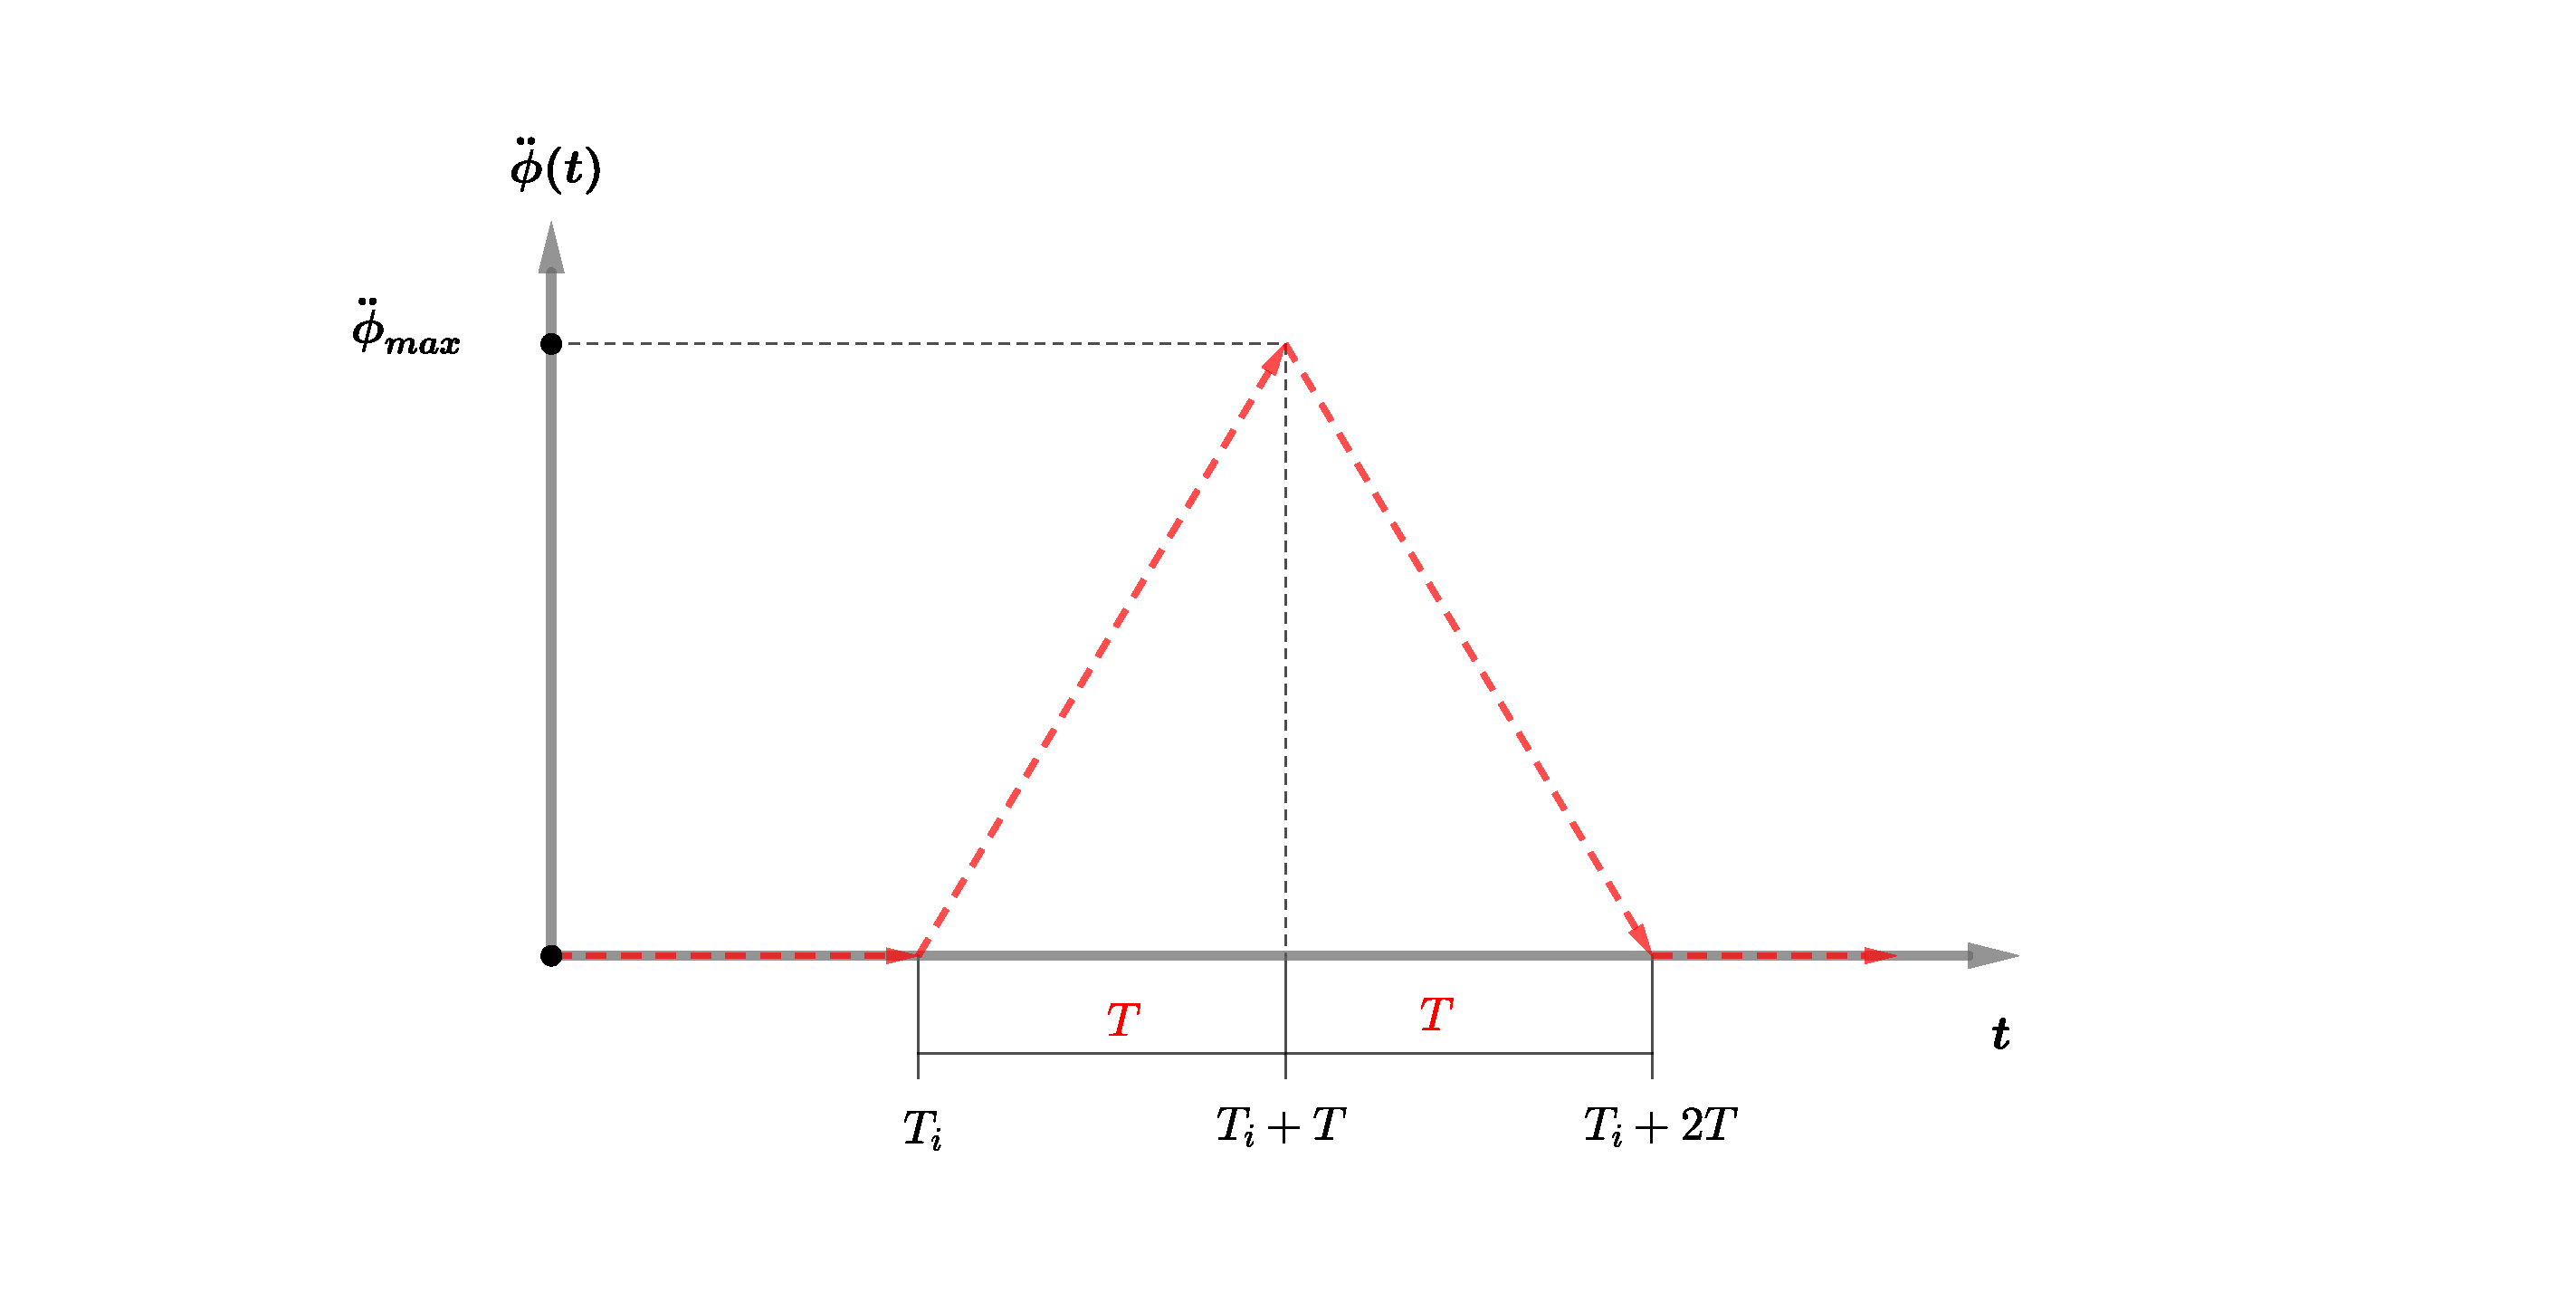
\includegraphics[scale=0.45,trim={6.5cm 2cm 10cm 2cm},clip]{Imagenes/anglepp_function.pdf}
\caption{Función por parte de la aceleración del disco}
\label{fig:anglepp}
\end{figure}
Así, la función $\ddot{\phi}$ adquiere la forma:
\[ \ddot{\phi}(t) =
\begin{dcases}
	0																		&	t \leq T_i \\
	\left(\frac{\omega_{max}}{T^2}\right)\left(t - T_i\right)				&	T_i < t \leq T_i + T\\
	\left(\frac{\omega_{max}}{T}\right)\left(2 - \frac{t - T_i}{T}\right)	&	T_i + T < t \leq T_i + 2T\\
	0																		&	T_i + 2T < t\\
\end{dcases} 
\]
Para obtener la función de la velocidad $\dot{\phi}(t)$ se debe integrar la función anterior, donde las constantes de integración se obtienen por los valores extremos conocidos, es decir, $\dot{\phi}(T_i) = 0$ y $\dot{\phi}(T_i + 2T) = \omega_{max}$. Entonces, la función se define como:
\[ \dot{\phi}(t) =
\begin{dcases}
	0																												&	t \leq T_i \\
	\left(\frac{\omega_{max}}{2T^2}\right)\left(t^2 - 2T_i\cdot t + T_i^2\right)									&	T_i < t \leq T_i + T\\
	\left(\frac{\omega_{max}}{T}\right)\left(2t - 2T_i - 3T + \frac{4T^2 - T_i^2 - t^2 + 2T_i\cdot t}{2T}\right)	&	T_i + T < t \leq T_i + 2T\\
	\omega_{max}																									&	T_i + 2T < t\\
\end{dcases} 
\]
El resultado de la función $\dot{\phi}(t)$, se muestra en la imagen \ref{fig:anglep}.
\begin{figure}[h]
\centering
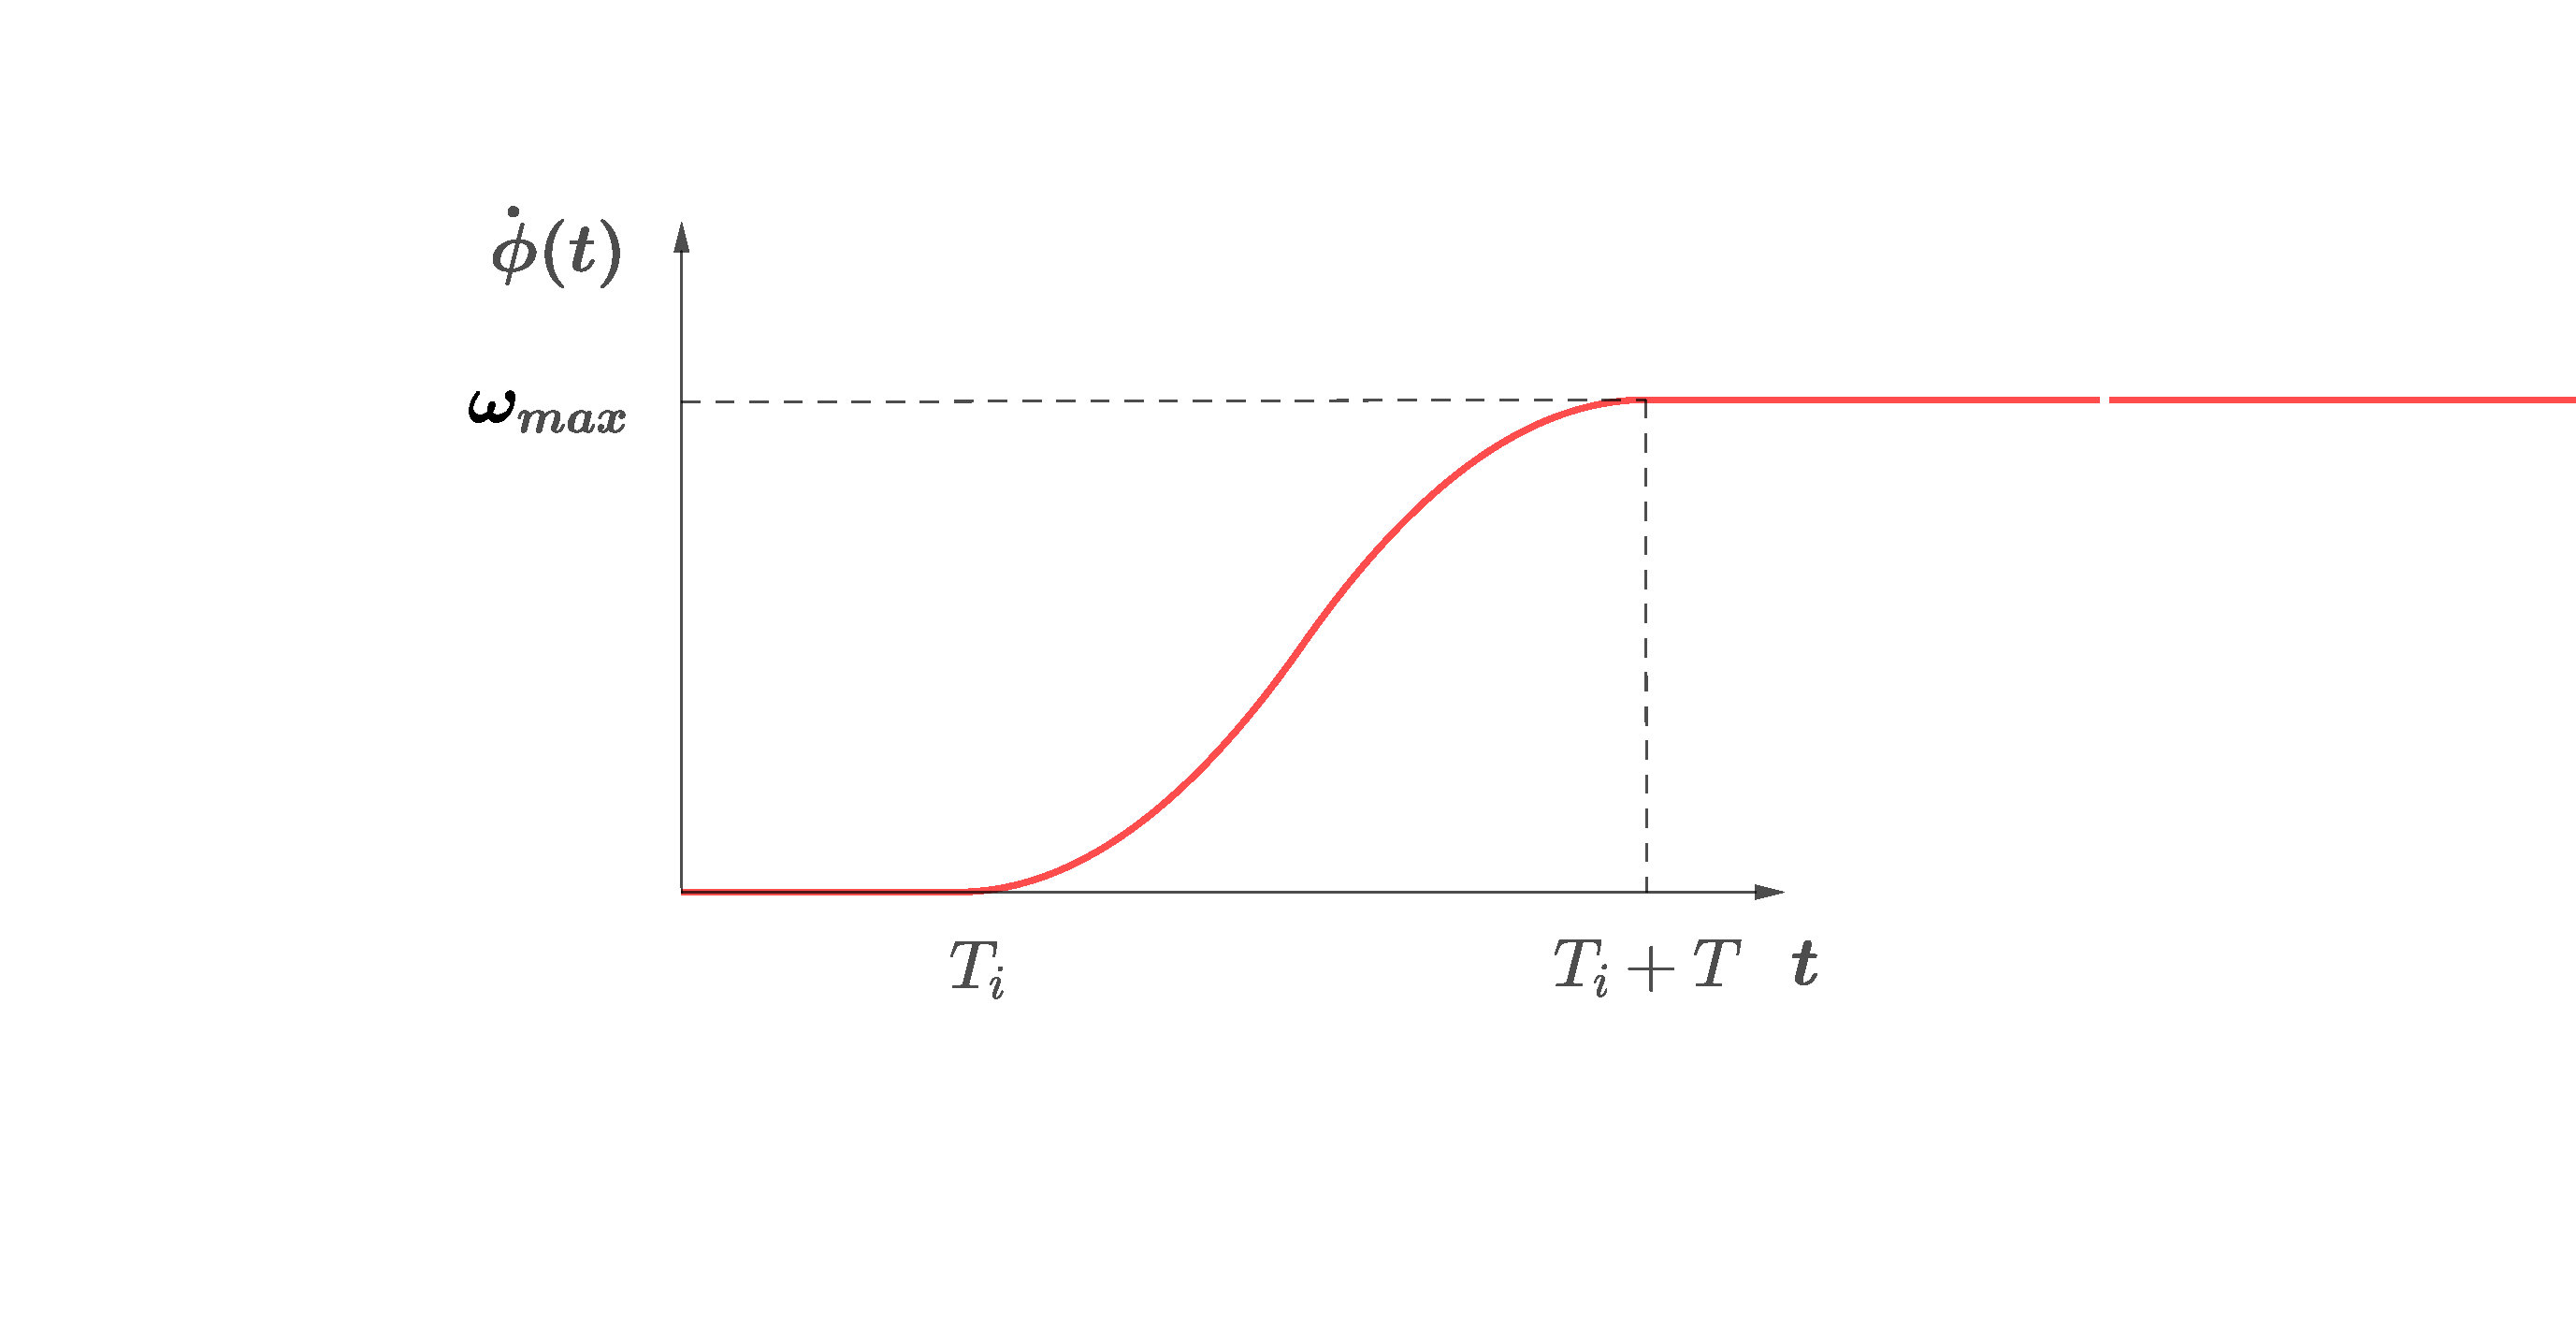
\includegraphics[scale=0.3,trim={5cm 0cm 4cm 0cm},clip]{Imagenes/anglep_function.pdf}
\caption{Función por parte de la velocidad angular del disco}
\label{fig:anglep}
\end{figure}

Para concluir, se repite el mismo procedimiento anterior para obtener la función $\phi (t)$, sin embargo, para conocer las constantes de integración, los puntos conocidos serán cuando $\phi(T_i) = 0$ y la igualdad de la función en el punto $T_i + T$. Así, es obtiene:
\[ \phi (t) =
\begin{dcases}
	0																									&	t \leq T_i \\
	\left(\frac{\omega_{max}}{6T^2}\right)\left(t^3 - 3T_i\cdot^2 t + 3T_i^2\cdot t - T_i^3\right)		&	T_i < t \leq T_i + T\\
	\Phi_3																								&	T_i + T < t \leq T_i + 2T\\
	\omega_{max}\, t - \omega_{max}(T + T_i)															&	T_i + 2T < t\\
\end{dcases} 
\]
La función $\phi_3$ correspondiente al dominio cuando $t$ es mayor $T_i + T$ y menor a $T_i  + 2T$ es:
\begin{multline*}
\Phi_3 = \left(\frac{\omega_{max}}{T}\right)\left(t^2 - 2T_i\cdot t - 3T\cdot t + \left(\frac{1}{2T}\right)\left(4T^2\cdot t - T_i^2\cdot t - \frac{t^3}{3} + T_i\cdot t^2\right)\right)\dots \\
 + \left(\frac{1}{6T^2}\right) \left(2\omega_{max}T^3 + 6\omega_{max}T^2T_i + 6\omega_{max}T\,T_i + \omega_{max}T_i^3\right)
\end{multline*}

Para el desarrollo de este trabajo, el tiempo de retraso de la aceleración del disco será de $T_i=2$, instante en el que la barra se encuentra en un estado de reposo en consecuencia del valor de los amortiguamientos $c_1$ y $c_2$. Por otro lado, se definirá $T = 2,5$ como un valor que logra suavizar la aceleración, pero sin dilatar en exceso la llegada al punto de velocidad máxima. Finalmente, $\omega_{max}\,$ el valor por defecto corresponderá a la velocidad actual de la máquina de 25 [rad/s] (1500 revoluciones por minuto), sin embargo, este se puede variar dependiendo de los resultados que se deseen obtener. 

\subsection{Solución del modelo}
Para resolver el sistema de ecuaciones que se obtuvo en \ref{eq:mov_matriz}, se utilizó el solver de ecuaciones diferenciales ordinarias de MATLAB, ode45, que se basa en el método de Runge-Kutta con un espacio de tiempo variable para resolver sistemas de EDOs de primer orden y con condición inicial. 

Es necesario ingresar datos de entrada que permitan resolver el sistema. Primero se debe escoger la configuración de contrapesos $m_1$ y $m_2$ a partir de la tabla de cargas. El segundo de ellos es el tiempo que define los límites de integración de la función, el que se escogerá según la cantidad de información que se desee obtener. En tercer lugar, se deben ingresar los valores de la condición inicial correspondiente a cada variable. Por último, es opcional añadir valores de tolerancia relativa y absoluta.

Al ser el sistema de ecuaciones de segundo orden, es necesario realizar un cambio de variables para poder resolverlo. Se añadirán las nuevas variables $\gamma$ y $\beta$, realizando la siguiente derivación:
\[ \left. 
\begin{array}{ll}
	\gamma = \dot{y}\\
	\beta = \dot{\theta}\\
\end{array}
\right\}
\begin{array}{ll}
	\ddot{y} &= \dot{\gamma}\\
	\ddot{\theta} &= \dot{\beta}\\
\end{array}\]
Para esto es necesario despejar los valores de $\ddot{y}$ y $\ddot{\theta}$, entonces la función a resolver estará dada por los elementos $(\gamma, \dot{\gamma}, \beta, \dot{\beta})$ y los resultados obtenidos serán $(y, \dot{y}, \theta, \dot{\theta})$. A partir de los resultados, es posible calcular la fuerza sobre la probeta utilizando la deformación $y_2$ y la constante de rigidez $k_2$.
\begin{equation}\label{eq:fuerza_probeta}
	F(t) = k_2 \cdot y_2 = k_2(y + l_2\theta)
\end{equation}

\subsection{Matriz de carga sobre la probeta según velocidad del motor}
Una vez que se puede resolver el sistema de ecuaciones para un configuración y velocidad del motor específica, entonces es posible obtener una matriz del valor de la fuerza máxima ($F_{max}$), media ($F_m$) y su amplitud ($F_a$) para cada una de las configuraciones existentes en la tabla de carga a una velocidad angular $\,\omega_{max}\,$ determinada.

Para esto se itera la solución anterior para cada una de las 201 configuraciones de contrapeso existentes para distintas velocidades. De estas iteraciones se almacenan los valores de $F_{max}$, $F_m$, $F_a$, la diferencia de masa de los contrapeso $\Delta m$ y la multiplicación entre la masa total $M_a$ y la excentricidad del centro de masa del disco $e_{ga}$.

\subsubsection{Carga máxima, media y amplitud}
Los información que se busca de estos resultados corresponde a la carga que es producto de la fuerza del disco desbalanceado, es decir, $F_d(t)$. Producto del comportamiento con el que se diseñó el modelo donde el sistema se deja caer hasta su posición de equilibrio,  se utiliza una variable auxiliar $F_{aux}$ que extrae los datos de $F(t)$ desde el inicio de la aceleración angular del disco hasta el final de la integración para evitar que las fuerzas de la transición entre la posición inicial y el reposo den resultados incorrectos. Así, la carga máxima, media y la amplitud se definen:
\begin{gather} 
	F_{max} = \text{max}(|F_{aux}|) \label{eq:f_max}\\
	F_m = \frac{\text{max}(F_{aux}) + \text{min}(F_{aux})}{2} \label{eq:f_m}\\
	F_a = \frac{\text{max}(F_{aux}) - \text{min}(F_{aux})}{2} \label{eq:f_a}
\end{gather}

\section{Simulación de cargas}

